%% Last modified: Time-stamp: <2011-06-16 23:18:48 (srdbadmin)>
\documentclass[letterpaper,review,authoryear,12pt]{myelsarticle}
\usepackage{amssymb}
\usepackage{pdflscape}
\usepackage{longtable}
\usepackage{graphicx}
\usepackage{paralist}
\usepackage{comment}
\usepackage{color}
\usepackage[left=3cm,top=3cm,right=3cm,bottom=3cm,nohead]{geometry}
\usepackage{booktabs}
\usepackage{url}
\usepackage[none]{hyphenat}  %% no hyphenation, to facilitate conversion to Word
\usepackage{microtype} %% no ligature, to facilitate conversion to Word
\DisableLigatures{encoding = *, family = * }

\begin{document}

\begin{frontmatter}
\title{Database contents for the Abstract, Results, Tables and Figures of the Fish and Fisheries paper 2011 resubmission}
\date{\today}
\end{frontmatter}

%\newpage
\section*{Abstract}

Data used to assess the status of individual fish stocks varies from
very little information on many of the world's artisanal fisheries, to
commercial landings, research surveys, and sophisticated population
dynamics models that integrate many sources of information.  Previous
evaluations of the state of global fisheries have used catch data,
which may be poor proxies for fish stock abundances. A global
compilation of stock assessment data in the mid-1990s enabled
substantial syntheses of stock status; however its focus was on
stock-recruitment relationships and it is now 15 years out of date. To
facilitate contemporary syntheses, we have assembled a new database,
the RAM Legacy Database, of the most intensively studied commercially
exploited marine fish stocks, including time series of total biomass,
spawner biomass, recruits, fishing mortality, and catch; reference
points; and ancillary information on the life history, management, and
assessment methods for each stock.  Here, we present the first
overview of this database and use it to evaluate the knowledge-base
for assessed marine species.  Assessments were assembled for
323 stocks (287 fish species
representing 45 families, and
36 invertebrate species representing
12 families), including 8 of the world's 10
largest fisheries. Assessments were obtained from 18 national and
international management institutions, with most coming from North
America, Europe, Australia, New Zealand and the high seas.  Overall,
58\% of stocks are below $B_{msy}$, and 30\% have exploitation levels above
$U_{msy}$.  Assessed marine fish stocks comprise a relatively small
proportion of harvested taxa (24\%), and an even smaller proportion of
marine fish biodiversity (1\%).


%Globally, stock assessments were found
%for 323 stocks (287 species
%of fishes representing 45 families and
%36 species of invertebrates representing
%12 families), from 18
%national and international
%management institutions.

\noindent Keywords: marine fisheries, meta-analysis, population dynamics models, relational database, stock assessment, synthesis.

%with XX\% coming from north temperate regions (North
%Atlantic, North Pacific)
%\noindent Keywords: marine fisheries, meta-analysis, population dynamics models, relational database, stock assessment, synthesis.
%\newpage

%  Geographic differences in assessment
%methods show that Statistical Catch at Age (SCA) models are widely
%used by the west coast of the U.S. (XX percent of assessments),
%regional fishery management organizations in the Pacific (XX percent
%of assessments), and New Zealand (XX percent of assessments); the east
%coast of the U.S. is transitioning from Virtual Population Analysis
%(VPA) to SCA (XX percent of assessments conducted since 2000 have used
%SCA); while VPA is still the dominant assessment
%technique in western Europe (XX percent of assessments).

\section*{Results}
\subsection*{Summary}
\noindent
Total number of proper stocks assessments: 331, from 295 marine fish populations and 36
invertebrate populations.

\subsection*{Taxonomy}
\noindent

Number of species in FishBase: 12339 (from 54 orders) \\
Number of species in SAUP: 925 (from 36 orders)\\
Number of species in RAM Legacy: 163 (from 58 families and 20 orders) \\
RAM Legacy contains 18\% of SAUP and 1\% of FishBase species\\
Top 5 taxonomic orders in RAM Legacy: Gadiformes (n=70), Perciformes (n=65), Pleuronectiformes (n=53), Scorpaeniformes (n=41), Clupeiformes (n=36) \\

\subsection*{Timespan}
\noindent
Number of assessments with catch timeseries: 313.\\
Number of assessments with recruitment timeseries: 274.\\
Number of assessments with spawning stock biomass timeseries: 280.\\

Together these comprise time series of
catch/landings for 313 stocks (95\%),
SSB estimates for 280 stocks (85\%), and recruitment estimates for
274 stocks (83\%).

The median lengths of catch/landings, SSB, and recruitment timeseries
were 39, 34, and 33
years, respectively.  The time period covered by 90\% of assessments
is: catch/landings (1966-2007), SSB
(1972-2007), recruitment (1971-2006), while that
covered by 50\% of assessments is: catch/landings
(1983-2004), SSB (1985-2005), recruitment
(1984-2003)
 
\subsection*{Assessment methodologies and reference points}
\noindent
The three most common assessment methods were
Statistical catch-at-age/length models (n=169), Virtual Population Analyses (n=92) and
Biomass dynamics model (n=45). Regionally, Virtual Population Analysis
(VPA) is still the most common assessment model for European stocks
(71\% of 63 assessments),
Canada (56\% of 26
assessments) and Argentina (83\% of
6 assessments), whereas statistical catch-at-age
and -length models are more common for the United States
(67\% of 138 assessments),
Australia (82\% of 17
assessments) and New Zealand (76\% of
29 assessments).

Biomass- or exploitation-based reference points were available for
262 (82\%) and
224 (69\%)
assessments, respectively.

\subsection*{Stock status}
\noindent

MSY-related reference points were avaialble for
113 stocks
(3 invertebrates) and estimated
for 102 additional stocks
(15 invertebrates), for a total of
215 stocks.

Of the
215 stocks presented in
the fried egg, 113 and
102 of the biomass reference points and
83 and
132 of the exploitation reference
points come from assessments and from surplus production model fits,
respectively.

To identify potential biases arising from using BRPs
derived from surplus production models we computed a contingency table
of status classification for stocks that have both assessment- and
Schaefer-derived BRPs (Table S2). Surplus production models correctly
classified ratios of current biomass to BRPs in
77\% of cases (for 60
of 78 assessments) and 64\%
of cases for exploitation BRPs (for 28 of
44 assessments).

Overall, 59\% of stocks are estimated
to be below their biomass-related MSY BRP, that is $B_{curr}<B_{msy}$,
and 31\% are estimated to be above
their exploitation-related MSY BRP, $U_{curr}>U_{msy}$
(n=215 stocks total.
Of the stocks for which biomass is currently estimated to be below
$B_{msy}$, 54\% have had their
exploitation rate reduced below $U_{msy}$, suggesting potential for
recovery. The remaining
46\% of these stocks however,
still have excessive exploitation rates. On a positive note,
41\% of all stocks are estimated to
be above $B_{msy}$, and 91\%
of the stocks above $B_{msy}$ also have $U_{current}$ below $U_{msy}$.


\subsection*{Global fisheries}

\subsection*{Management bodies and geography}
\noindent
Number of assessments from NMFS: 138 (81 with reference points, 41 (51 \%) are below $B_{msy}$, 63 (78 \%) are below $U_{msy}$, ) \\

Number of assessments from ICES: 63 (48 with reference points, 39 (81 \%) are below $B_{msy}$, 22 (46 \%) are below $U_{msy}$, ) \\

Number of assessments from ICES: 63 (23 with Blim and Flim reference points, 7 are below $B_{lim}$ and above $F_{lim}$, 1 are above $B_{lim}$ and above $F_{lim}$, 11 are above $B_{lim}$ and below $F_{lim}$ and 4 are below $B_{msy}$ and below $F_{lim}$.

Number of assessments from MFish: 29 (28 with reference points, 11 (39 \%) are below $B_{msy}$, 22 (79 \%) are below $U_{msy}$, ) \\
Number of assessments from DFO: 26 (14 with reference points, 12 (86 \%) are below $B_{msy}$, 13 (93 \%) are below $U_{msy}$, ) \\
Number of assessments from AFMA: 17 (11 with reference points, 7 (64 \%) are below $B_{msy}$, 7 (64 \%) are below $U_{msy}$, ) \\
Number of assessments from DETMCM: 14 (6 with reference points, 3 (50 \%) are below $B_{msy}$, 5 (83 \%) are below $U_{msy}$, ) \\

The status of exploited marine stocks, as estimated from biomass- and
exploitaion-BRPs, varied widely depending on the management body. Most European stocks (managed by
ICES) have biomasses less than $B_{msy}$
(81\%), and over half of these
stocks (59\%) still
have exploitation rates exceeding $U_{msy}$. Canadian stocks (managed
by DFO) also had low biomass (86\%
$< B_{msy}$), but all but one of these has had its exploitation rate
reduced below $U_{msy}$. In contrast, about half
(49\%) of U.S. stocks (managed by
NMFS) are estimated to still be above $B_{msy}$, and of the
41 stocks that are below $B_{msy}$
63\% have exploitation
rates below $U_{msy}$. In the New
Zealand and Australian waters, stocks managed by MFish and AFMA are
above $B_{msy}$ in 61\% and
36\% of cases, respectively. For
the stocks grouped as ``Atlantic'' in the fried eggs we
found that 6 of the
10 ICCAT stocks and
6 of the
10 of NAFO stocks were below $B_{msy}$ .

%Number of assessments from ICES: 63.\\
%Number of assessments from MFish: 29.\\
%Number of assessments from DFO: 26.\\
%Number of assessments from AFMA: 17.\\
%Number of assessments from DETMCM: 14.\\


Assessments were available for 27 LMEs, with the greatest number of
assessed stocks coming from Northeast U.S. Continental Shelf (n=58),
California Current (n=35), New Zealand Shelf (n=29),
Gulf of Alaska (n=27), Celtic-Biscay Shelf (n=26), East Bering Sea (n=21)
and Southeast U.S. Continental Shelf (n=19).

The proportion of stocks below $B_{msy}$ and below $U_{mys}$ varies considerably by management body. 

ICES has 48 assessments in Table 4,
39
(81\%) of which are below
$B_{msy}$ and 22 are below
$U_{msy}$.

\subsection*{Stock status by taxonomic orders}

Of the 48 stocks for Gadiformes, 15 are below $B_{msy}$ and above $U_{msy}$, 2 are above $B_{msy}$ and above $U_{msy}$, 9 are above $B_{msy}$ and below $U_{msy}$ and 22 are below $B_{msy}$ and below $U_{msy}$.

Of the 46 stocks for Perciformes, 15 are below $B_{msy}$ and above $U_{msy}$, 1 are above $B_{msy}$ and above $U_{msy}$, 17 are above $B_{msy}$ and below $U_{msy}$ and 13 are below $B_{msy}$ and below $U_{msy}$.

Of the 38 stocks for Pleuronectiformes, 14 are below $B_{msy}$ and above $U_{msy}$, 1 are above $B_{msy}$ and above $U_{msy}$, 18 are above $B_{msy}$ and below $U_{msy}$ and 5 are below $B_{msy}$ and below $U_{msy}$.

Of the 25 stocks for Scorpaeniformes, 2 are below $B_{msy}$ and above $U_{msy}$, 1 are above $B_{msy}$ and above $U_{msy}$, 14 are above $B_{msy}$ and below $U_{msy}$ and 8 are below $B_{msy}$ and below $U_{msy}$.

Of the 23 stocks for Clupeiformes, 4 are below $B_{msy}$ and above $U_{msy}$, 2 are above $B_{msy}$ and above $U_{msy}$, 7 are above $B_{msy}$ and below $U_{msy}$ and 10 are below $B_{msy}$ and below $U_{msy}$.

Of the 12 stocks for Decapoda, 5 are below $B_{msy}$ and above $U_{msy}$, 1 are above $B_{msy}$ and above $U_{msy}$, 2 are above $B_{msy}$ and below $U_{msy}$ and 4 are below $B_{msy}$ and below $U_{msy}$.


\subsection*{Stock status by Mean Trophic Level}
Of the 26 stocks of MTL between 2 and 3 , 10 are below $B_{msy}$ and above $U_{msy}$, 1 are above $B_{msy}$ and above $U_{msy}$, 7 are above $B_{msy}$ and below $U_{msy}$ and 8 are below $B_{msy}$ and below $U_{msy}$.

Of the 94 stocks of MTL between 3 and 4 , 19 are below $B_{msy}$ and above $U_{msy}$, 3 are above $B_{msy}$ and above $U_{msy}$, 38 are above $B_{msy}$ and below $U_{msy}$ and 34 are below $B_{msy}$ and below $U_{msy}$.

Of the 91 stocks of MTL above 4 , 27 are below $B_{msy}$ and above $U_{msy}$, 4 are above $B_{msy}$ and above $U_{msy}$, 35 are above $B_{msy}$ and below $U_{msy}$ and 25 are below $B_{msy}$ and below $U_{msy}$.

\subsection*{Stock status by Functional Grouping}
Of the 147 demersal stocks, 40 are below $B_{msy}$ and above $U_{msy}$, 4 are above $B_{msy}$ and above $U_{msy}$, 58 are above $B_{msy}$ and below $U_{msy}$ and 45 are below $B_{msy}$ and below $U_{msy}$.

Of the 49 pelagic stocks, 11 are below $B_{msy}$ and above $U_{msy}$, 3 are above $B_{msy}$ and above $U_{msy}$, 18 are above $B_{msy}$ and below $U_{msy}$ and 17 are below $B_{msy}$ and below $U_{msy}$.

Of the 18 invertebrates stocks, 7 are below $B_{msy}$ and above $U_{msy}$, 1 are above $B_{msy}$ and above $U_{msy}$, 4 are above $B_{msy}$ and below $U_{msy}$ and 6 are below $B_{msy}$ and below $U_{msy}$.


\section*{References}
\bibliographystyle{fishandfisheriesBST}
\bibliography{./fishfisheries}

\section*{Tables}

%First output Table 1 as generated from the database contents.
\begin{tiny}
% latex table generated in R 2.9.1 by xtable 1.5-6 package
% Mon Jun 21 15:34:31 2010
\begin{table}[ht]
\begin{center}
\caption{Number of assessments included in the RAM Legacy database}
\label{tab:mgmt}
\begin{tabular}{p{3cm}p{5cm}cc}
\textit{Country/Ocean} & \textit{Management Body} & \textit{Acronym} & \textit{No. stocks} \\ \midrule
Australia & Australian Fisheries Management Authority & AFMA &  16 \\ 
  Multinational & Commission for the Conservation of Antarctic Marine Living Resources & CCAMLR &   1 \\ 
  Argentina & Consejo Federal Pesquero & CFP &   6 \\ 
  South Africa & South African national management & DETMCM &  14 \\ 
  Canada & Department of Fisheries and Oceans & DFO &  22 \\ 
  Multinational & Inter-American Tropical Tuna Commission & IATTC &   2 \\ 
  Multinational & International Commission for the Conservation of Atlantic Tunas & ICCAT &  10 \\ 
  Multinational & International Council for the Exploration of the Sea & ICES &  63 \\ 
  Multinational & Indian Ocean Tuna Commission & IOTC &   1 \\ 
  Multinational & International Pacific Halibut Commission & IPHC &   1 \\ 
  New Zealand & Ministry of Fisheries & MFish &  29 \\ 
  Multinational & Northwest Atlantic Fisheries Organization & NAFO &   9 \\ 
  USA & National Marine Fisheries Service & NMFS & 139 \\ 
  Russia & Russian Federal Fisheries Agency & RFFA &   2 \\ 
  Multinational & South Pacific Regional Fisheries Management Organization & SPRFMO &   1 \\ 
  Multinational & Unknown management body & UNKNOWN &   1 \\ 
  USA & US state-level management & US State &   3 \\ 
  Multinational & Western and Central Pacific Fisheries Commission & WCPFC &   4 \\ 
   \hline
\end{tabular}
\end{center}
\end{table}

\end{tiny}

%Next output the different figures.
\section*{Figures}
\subsection*{Figure legends}

\noindent Figure 1. Orca plots showing the temporal coverage of (A)
catch/landings, (B) spawning stock biomass and (C) recruitment. The
temporal coverage for individual assessments is represented by thin
alternating black and grey horizontal lines in the main panels. Orca
plots are named because their distinctive shape is uncannily similar
to the individually-identifiable nicked and notched dorsal fins of
killer whales (orcas). Thick horizontal lines at the base of each main
panel represent the time periods which are present in 90\% (black) and
50\% (grey) of all series for that data type.  Subfigure histograms
contain the frequency of occurrence of the various timespans without
reference to time period. Solid and long-dash vertical lines within
the subfigures represent the median,
2.5\% and 97.5\% quantiles, respectively.\\

\noindent Figure 2. Map of Large Marine Ecosystems (LMEs) and
high seas areas (ovals) showing the number of stock assessments
present in the database for each area. This map illustrates the limited
spatial coverage of available stock assessments.\\

\noindent Figure 3. Comparison of the taxonomic diversity of marine
species as provided by FishBase (top panel), the coverage of catch
data as provided by the Sea Around Us database (middle panel) and the
new RAM Legacy database (bottom panel). The circle located near the
middle of the circular dendrogram represents kingdom Animalia and each
subsequent branching represents a different taxonomic group (Kingdom
to Phylum to Class to Order to Family to Genus to Species). The width
of each line is proportional to the square root of the number of
species in a branch. To facilitate the identification of the taxonomic
groups that are not presented in the catch and assessment data, the
FishBase branching pattern of the spoked dendrogram is maintained to
generate the other two dendrograms.  This figure only compares fish
and elasmobranch species present in FishBase. Additonal species of
molluscs and arthropods are present in both the Sea Around Us and RAM
Legacy databases but are not presented here.
\\


\noindent Figure 4. Current exploitation rate versus current biomass
for 213 individual stocks and for individual stocks grouped by
management unit. Exploitation is scaled relative to that which should
allow maximum sustainable yield ($U_{msy}$); biomass is scaled
relative to $B_{msy}$. Shades of grey indicate probability of
occurrence as revealed by a kernel density smooth function. Solid
circles indicate $B_{msy}$ and $U_{msy}$ that were obtained directly
from assessments; open circles indicate that they were estimated from
surplus production models. The panel labelled ``Atlantic'' includes
ICCAT and NAFO. This figure is an updated version of Fig 3B from
\citet{Worm:etal:2009:science}.
\\

\noindent Figure 5. Current exploitation rate versus current biomass grouped by the six taxonomic orders with the most assessments.
\\

\noindent Figure 6. Current exploitation rate versus current biomass grouped by mean trophic level.
\\

\newpage
\subsection*{Figures}

\begin{landscape}
\begin{figure}
\begin{center}
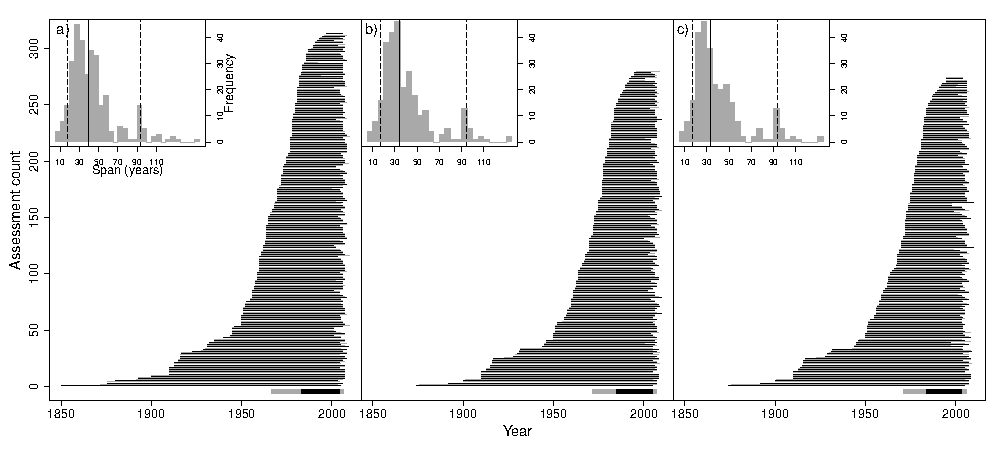
\includegraphics[width=8in]{/home/srdbadmin/srdb/projects/fishandfisheries/R/first-review/orca-plot.pdf}
\end{center}
\caption{ }\label{fig:orca}
\end{figure}
\end{landscape}

\begin{landscape}
\begin{figure}
\begin{center}
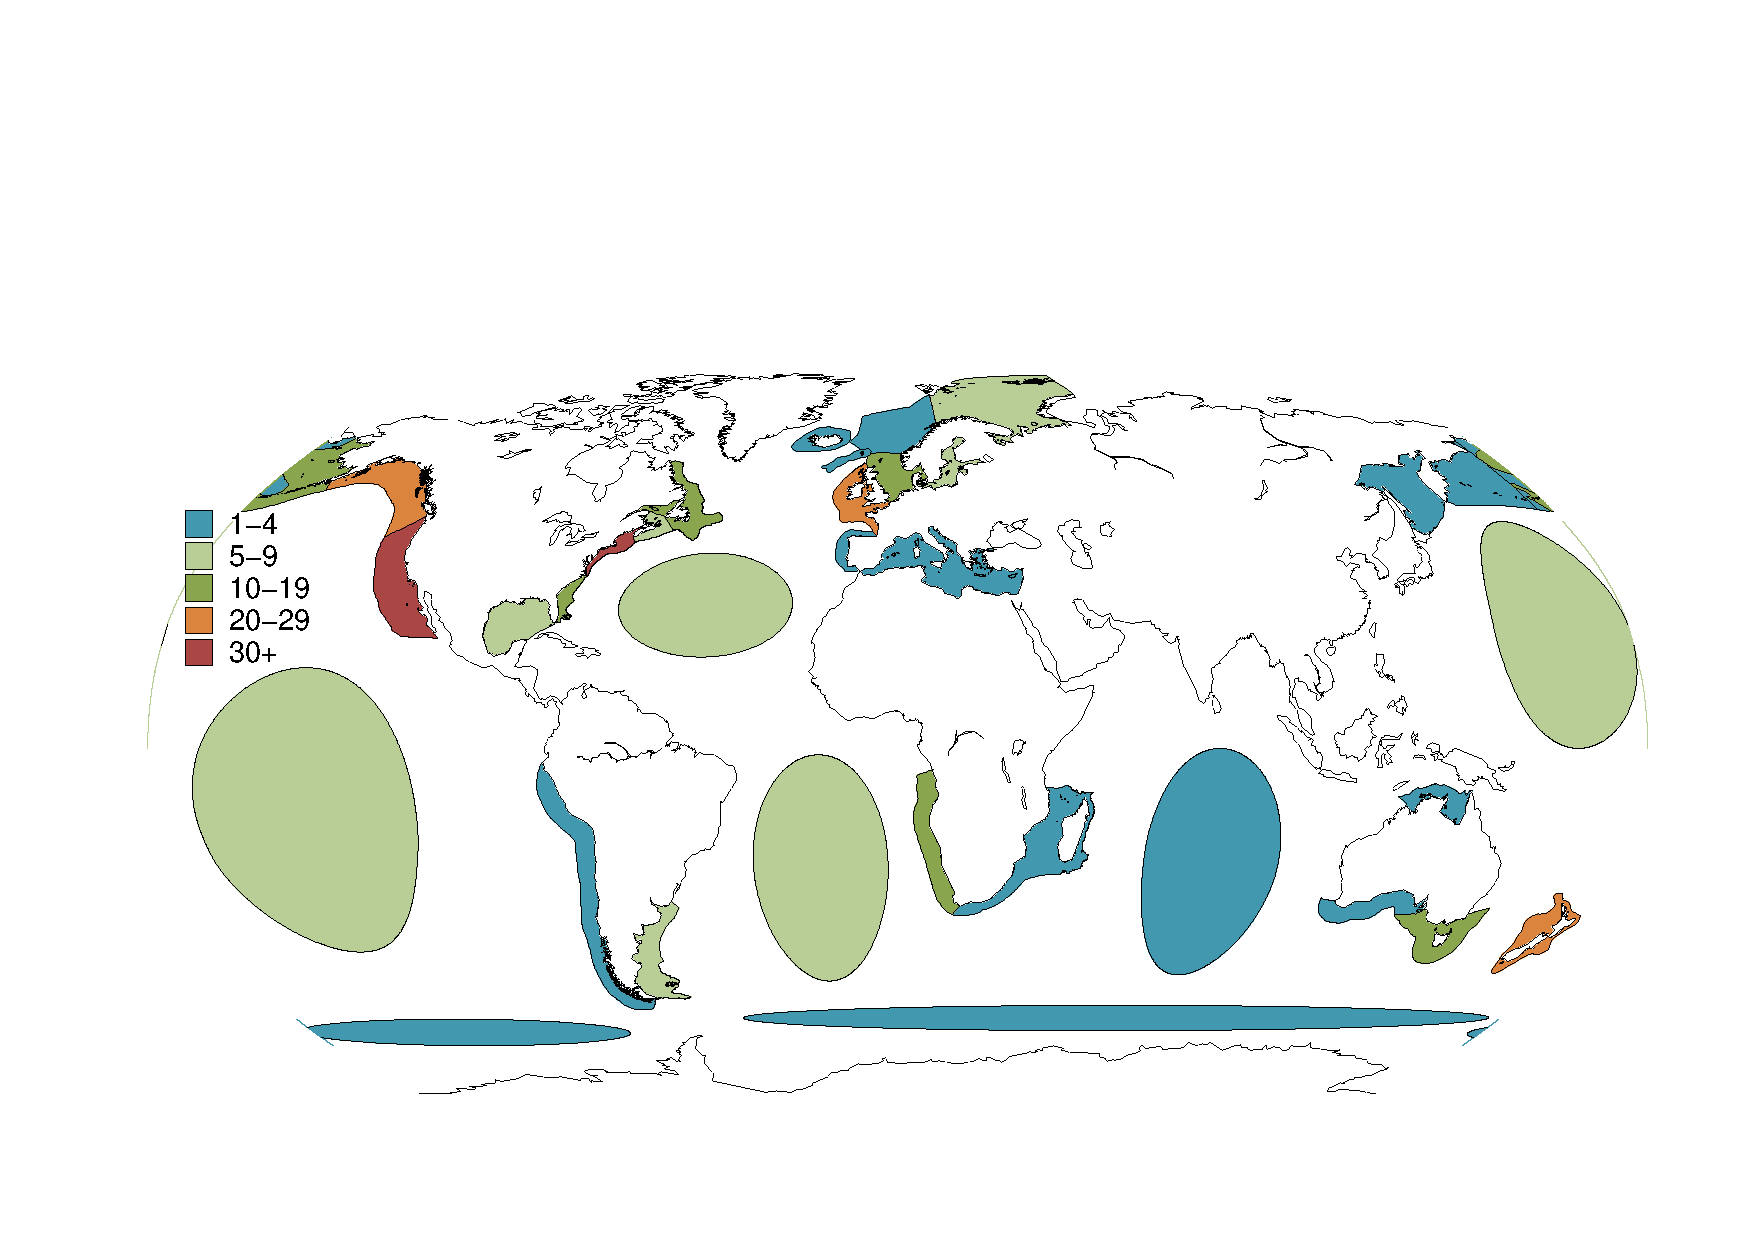
\includegraphics[width=9in]{/home/srdbadmin/srdb/projects/fishandfisheries/GMT/stocks-byLME.pdf}
\end{center}
\caption{ }\label{fig:lmes}
\end{figure}
\end{landscape}


\begin{figure}
\begin{center}
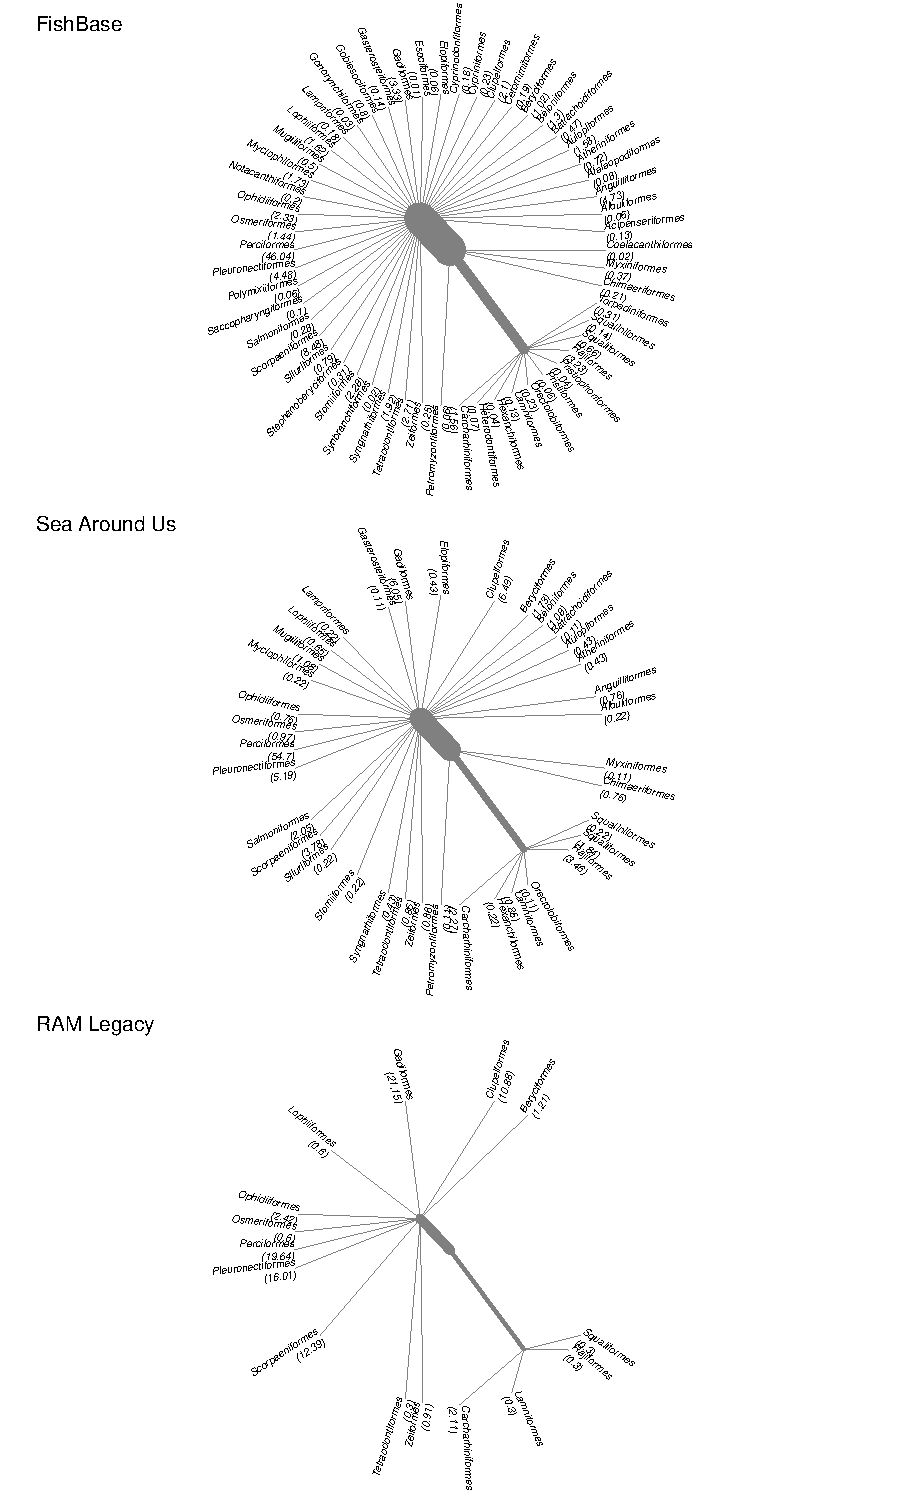
\includegraphics[height=8.5in]{/home/srdbadmin/srdb/projects/fishandfisheries/R/first-review/three-panel-phylo.pdf} % fishbase_saup_two_panel_phylo.pdf}
\end{center}
\caption{ }\label{fig:taxo:threepanel}
\end{figure}




%\begin{figure}
%\begin{center}
%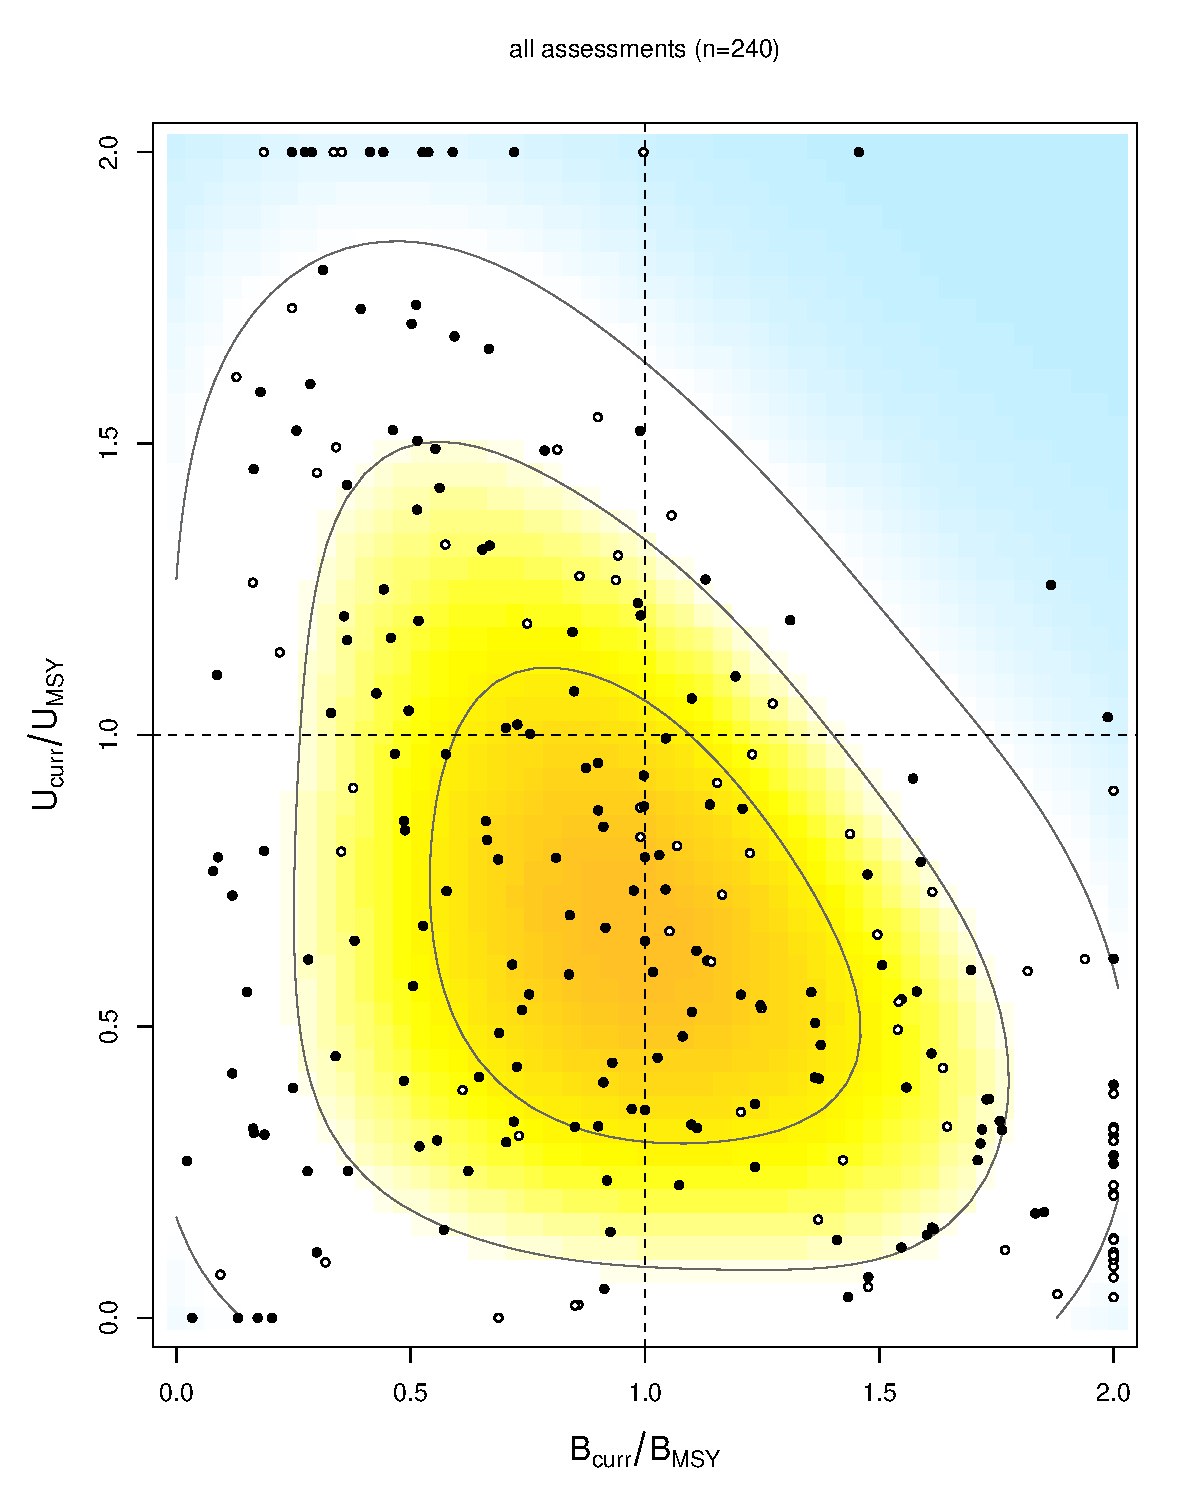
\includegraphics[width=15cm]{/home/srdbadmin/srdb/projects/fishandfisheries/R/first-review/friedegg-single.pdf}
%\end{center}
%\caption{ }\label{fig:friedegg}
%\end{figure}

%Some options for the management-level fried eggs.

%\begin{figure}
%\begin{center}
%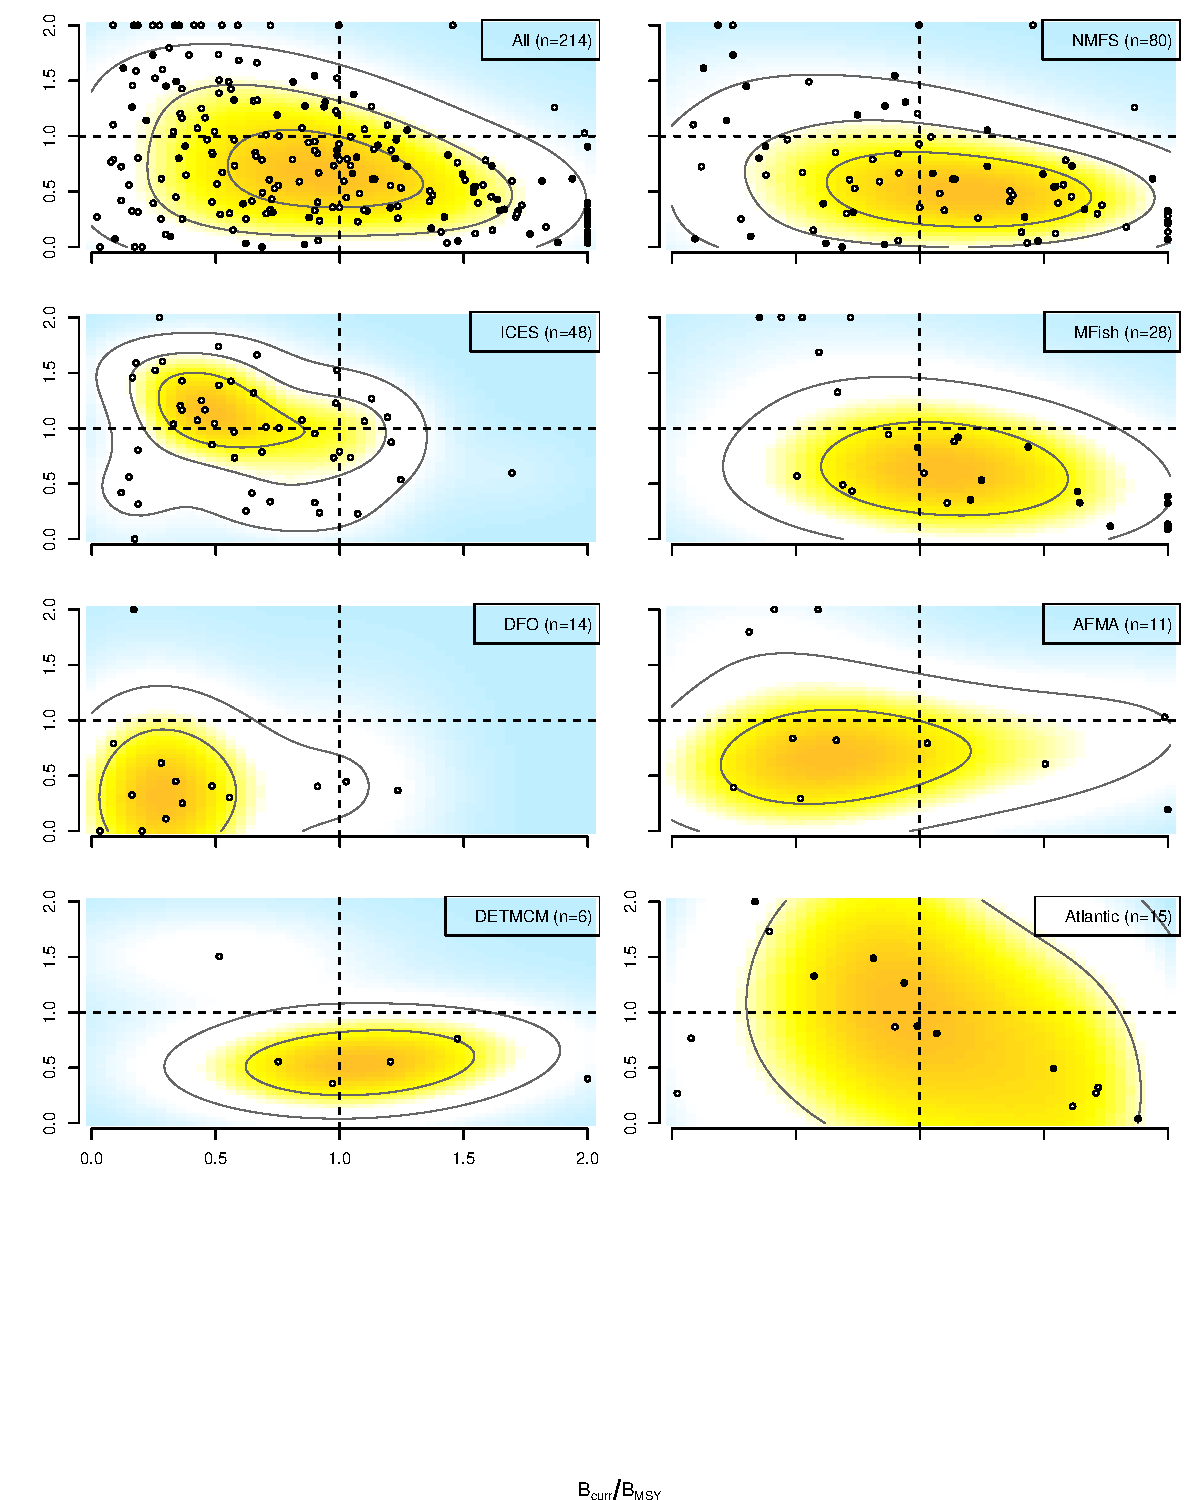
\includegraphics[width=15cm]{/home/srdbadmin/srdb/projects/fishandfisheries/R/first-review/friedegg-bymgmt.pdf}
%\end{center}
%\caption{Option 1 }\label{fig:friedegg}
%\end{figure}

%\begin{figure}
%\begin{center}
%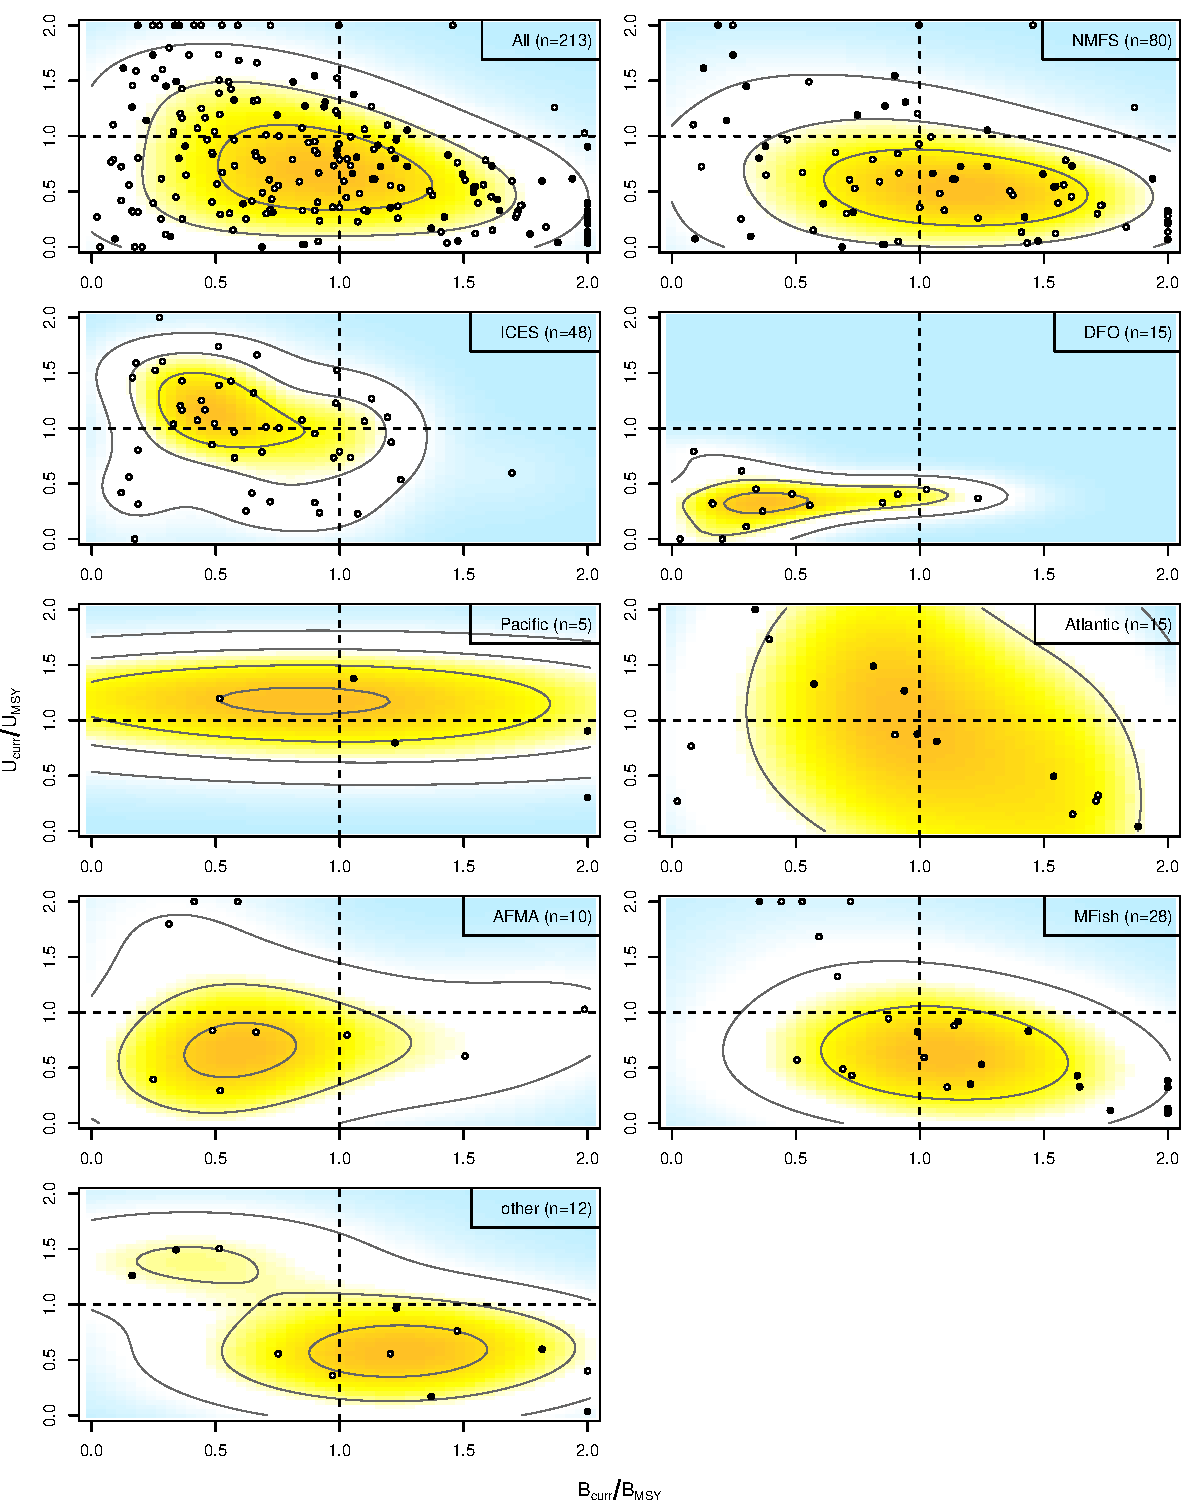
\includegraphics[width=15cm]{/home/srdbadmin/srdb/projects/fishandfisheries/R/first-review/friedegg-bymgmt-10plots.pdf}
%\end{center}
%\caption{Option 2 }
%\end{figure}

%\begin{landscape}
%\begin{figure}
%\begin{center}
%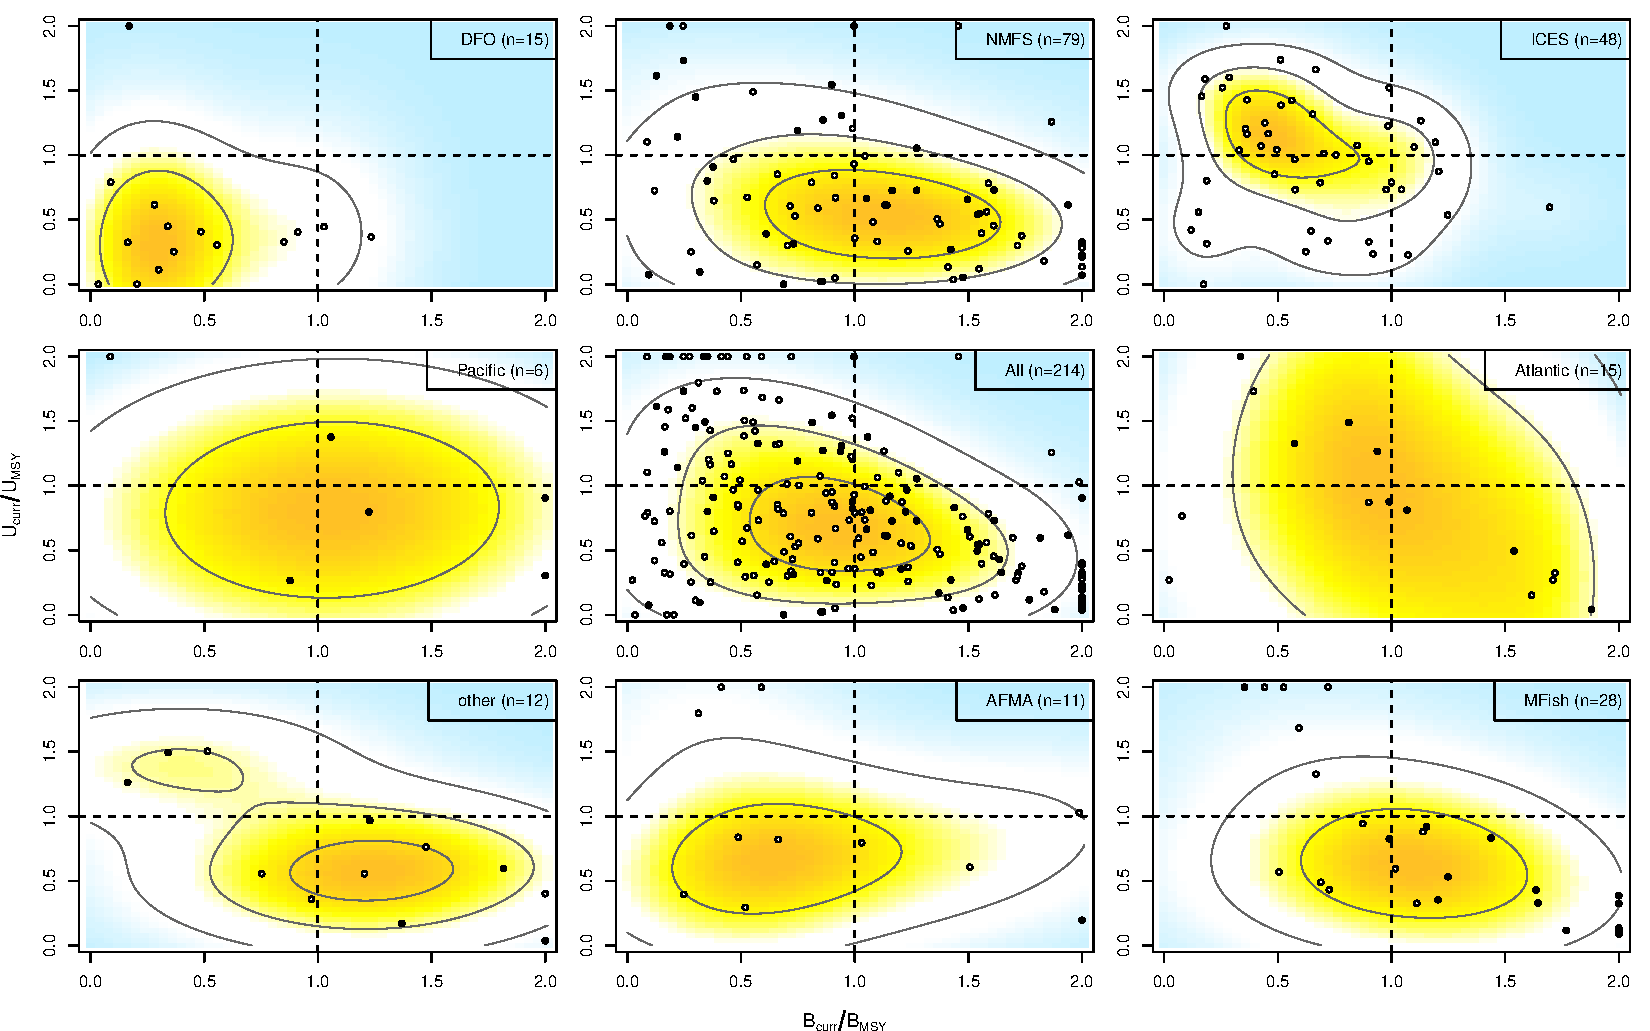
\includegraphics[width=9in]{/home/srdbadmin/srdb/projects/fishandfisheries/R/first-review/friedegg-9plots.pdf}
%\end{center}
%\caption{ Option 3}\label{fig:friedegg}
%\end{figure}
%\end{landscape}

\begin{landscape}
\begin{figure}
\begin{center}
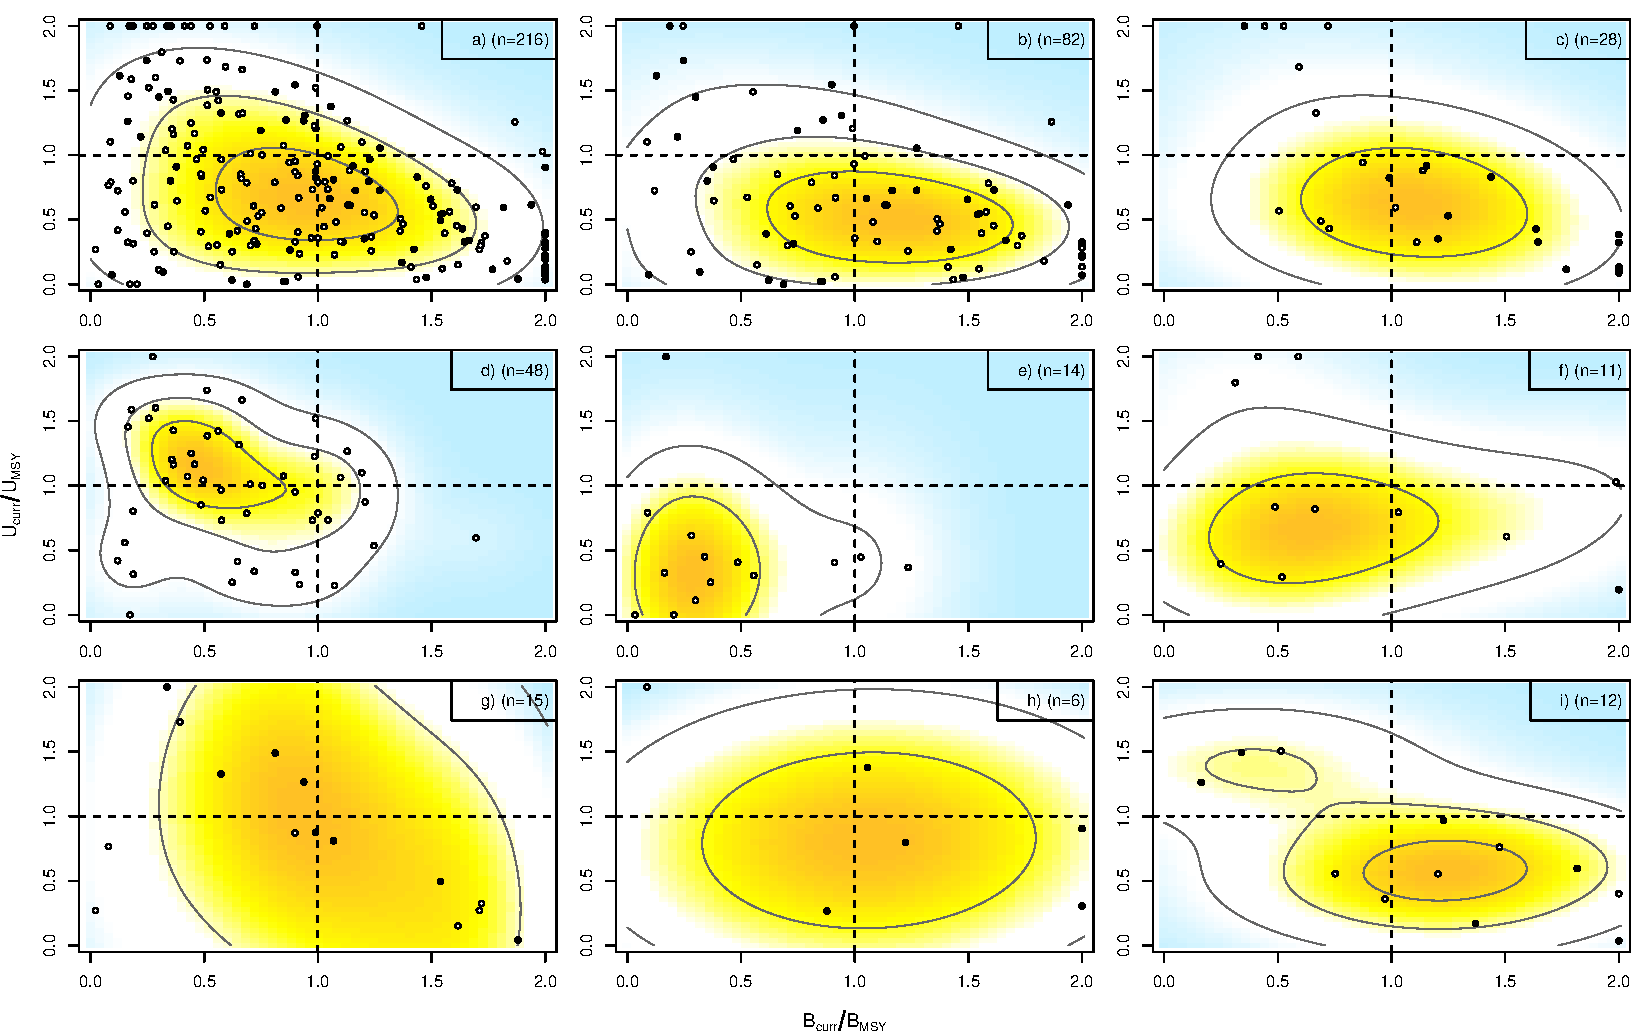
\includegraphics[width=9in]{/home/srdbadmin/srdb/projects/fishandfisheries/R/first-review/friedegg-9plots-fandf.pdf}
\end{center}\label{fig:friedegg}
%\caption{ Option 3}
\end{figure}
\end{landscape}

%For the top 6 taxonomic orders (Figure~\ref{fig:taxo}).
\begin{figure}
\begin{center}
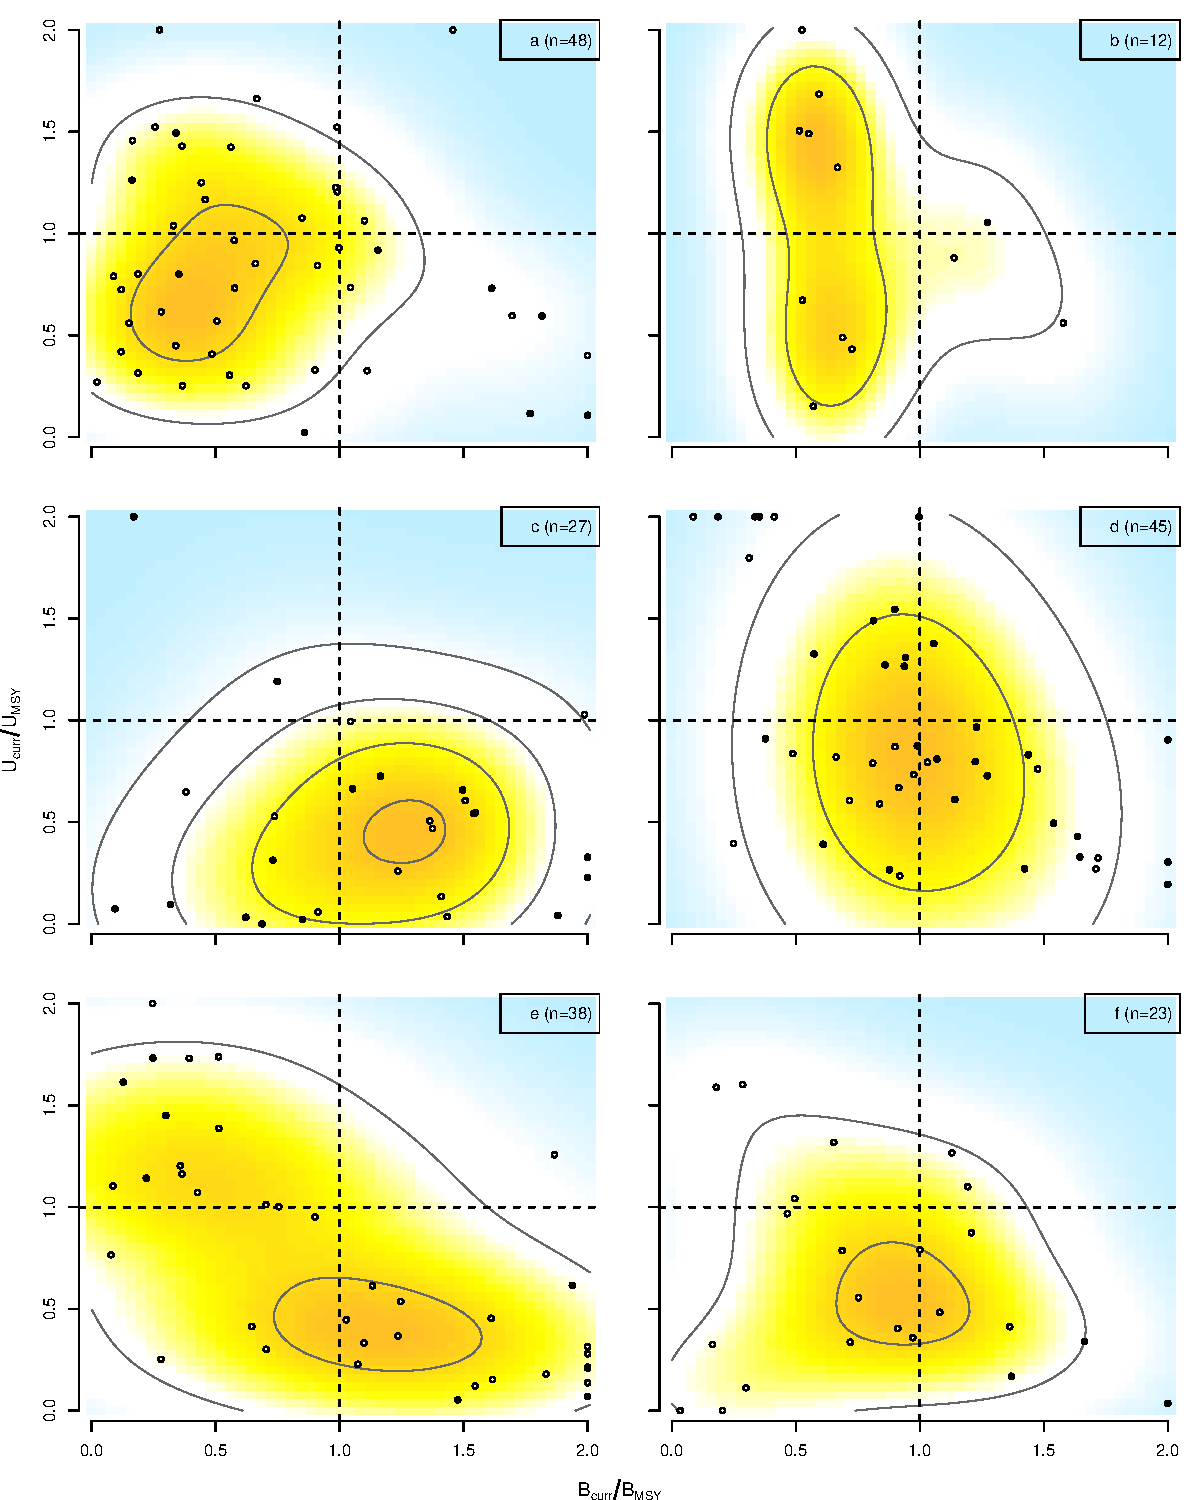
\includegraphics[width=15cm]{/home/srdbadmin/srdb/projects/fishandfisheries/R/first-review/friedegg-taxo.pdf}
\end{center}
\caption{Top 6 taxonomic orders. }
\label{fig:taxo}
\end{figure}

%By trophic level (Figure~\ref{fig:mtl}).
\begin{figure}
\begin{center}
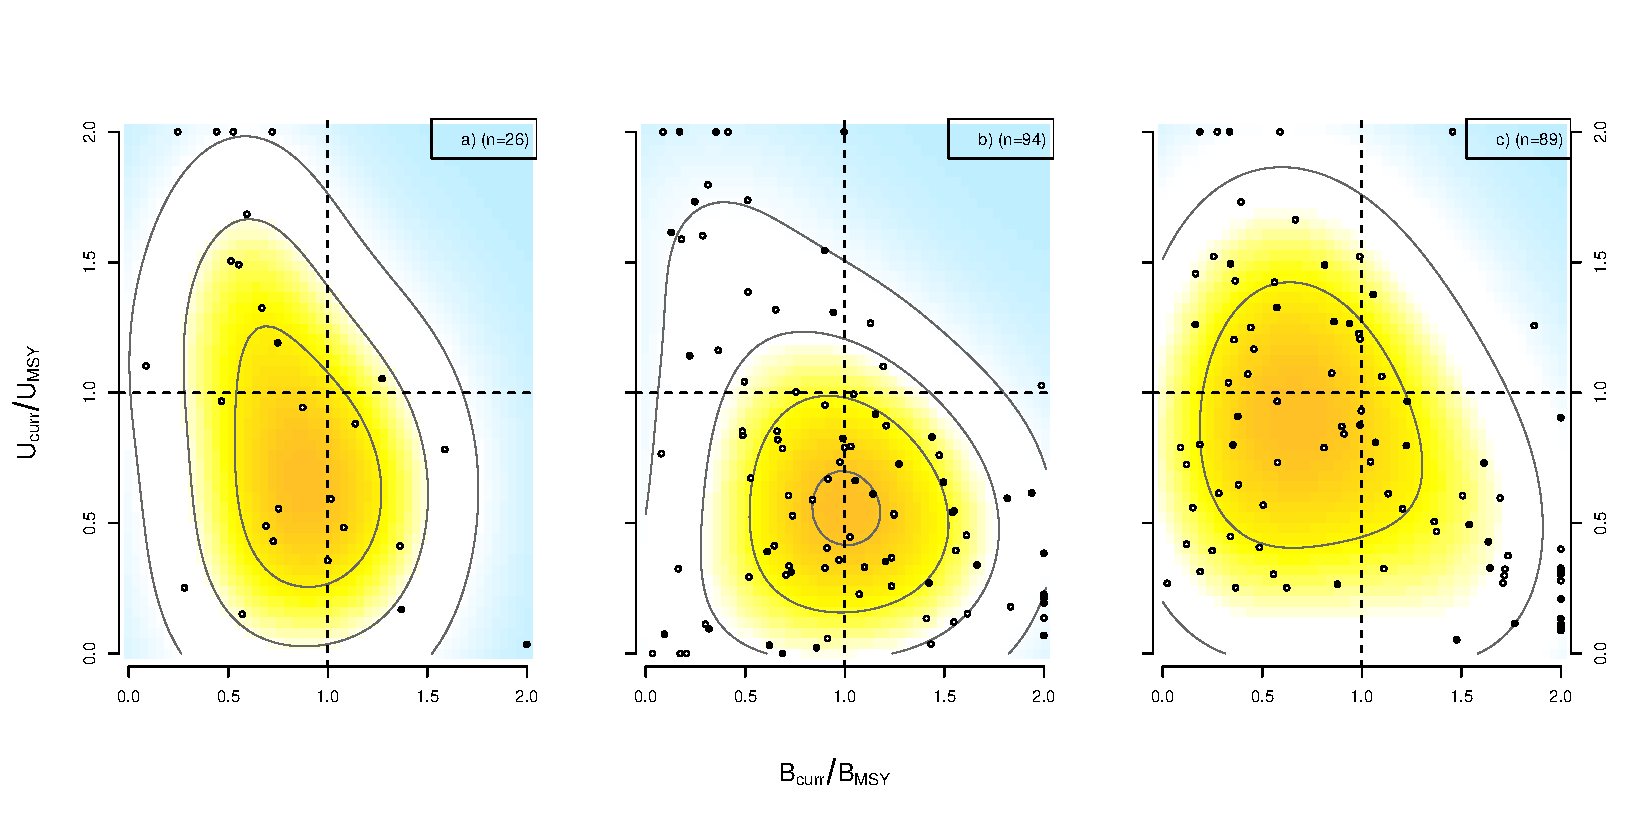
\includegraphics[width=15cm]{/home/srdbadmin/srdb/projects/fishandfisheries/R/first-review/friedegg-MTLs.pdf}
\end{center}
\caption{By mean trophic level (MTL).}
\label{fig:mtl}
\end{figure}







\begin{appendix}
Contents for Supplementary Materials

%Supplementary Table S2
% latex table generated in R 2.13.0 by xtable 1.5-6 package
% Thu May 19 14:38:14 2011
\begin{table}[ht]
\begin{center}
\begin{tabular}{ccc}
  \hline
 & SP U/Umsy $<$ 1 & SP U/Umsy $>$ 1 \\ 
  \hline
U/Umsy $<$ 1 &  20 &  14 \\ 
  U/Umsy $>$ 1 &   2 &   8 \\ 
  B/Bmsy $<$ 1 &  28 &   6 \\ 
  B/Bmsy $>$ 1 &  12 &  30 \\ 
   \hline
\end{tabular}
\caption{Contingency tables of stock status classification for biomass and exploitation reference points obtained from assessments and those derived from surplus production models. }
\label{tab:contingency}
\end{center}
\end{table}


%Supplementary Table S1
\begin{landscape}
\begin{tiny}
% latex table generated in R 2.9.1 by xtable 1.5-6 package
% Tue Jun 15 14:05:37 2010
\begin{longtable}{p{1.8cm}p{4cm}p{4cm}ccccp{1.9cm}c}
  \bottomrule \\ \multicolumn{2}{c}{Continued on next page} \endfoot \endlastfoot
Management & Stock ID & Scientific name & Timespan & Current year & B ratio & U ratio & From assessment & Ref. \\ \midrule \endhead
AFMA & Bight redfish Southeast Australia & \textit{Centroberyx gerrardi} & 1958-2007 &  &  &  &  & \cite{BIGHTREDDEEPFLATSE.pdf} \\ 
  AFMA & New Zealand ling Eastern half of Southeast Australia & \textit{Genypterus blacodes} & 1968-2007 & 2007 & 0.60 & 2.20 & no & \cite{NZLINGSE.pdf} \\ 
  AFMA & New Zealand ling Western half of Southeast Australia & \textit{Genypterus blacodes} & 1968-2007 &  &  &  &  & \cite{NZLINGSE.pdf} \\ 
  AFMA & Orange roughy Cascade Plateau & \textit{Hoplostethus atlanticus} & 1987-2006 & 2006 & 1.76 & 0.34 & no & \cite{CSIRO-Cascade-Plateau-Stock-Assessment-2006.pdf} \\ 
  AFMA & Orange roughy Southeast Australia & \textit{Hoplostethus atlanticus} & 1978-2007 & 2006 & 0.89 & 0.29 & no & \cite{OROUGHYSE.pdf} \\ 
  AFMA & Jackass morwong Southeast Australia & \textit{Nemadactylus macropterus} & 1913-2007 & 2007 & 0.25 & 1.80 & no & \cite{MORWONGSE.pdf} \\ 
  AFMA & Tiger flathead Southeast Australia & \textit{Neoplatycephalus richardsoni} & 1913-2006 & 2006 & 1.05 & 0.00 & no & \cite{TIGERFLATSE.pdf} \\ 
  AFMA & Northern Australia brown tiger shrimp & \textit{Penaeus esculentus} & 1970-2006 &  &  &  &  & \cite{NORTHPRAWNS.pdf} \\ 
  AFMA & Northern Australia grooved Tiger Prawn & \textit{Penaeus esculentus} & 1970-2006 &  &  &  &  & \cite{NORTHPRAWNS.pdf} \\ 
  AFMA & Deepwater flathead Southeast Australia & \textit{Platycephalus conatus} & 1978-2007 & 2006 & 1.33 & 0.61 & no & \cite{BIGHTREDDEEPFLATSE.pdf} \\ 
  AFMA & Tasmanian giant crab Tasmania & \textit{Pseudocarcinus gigas} & 1990-2007 & 2007 & 0.50 & 1.71 & no & \cite{JENSEN_TASGIANTCRAB_2008.pdf} \\ 
  AFMA & common gemfish Southeast Australia & \textit{Rexea solandri} & 1966-2007 & 2007 & 0.10 & 0.39 & no & \cite{GEMFISHSE.pdf} \\ 
  AFMA & Blue Warehou Eastern half of Southeast Australia & \textit{Seriolella brama} & 1984-2006 & 2006 & 0.17 & 0.84 & no & \cite{WAREHOUSE.pdf} \\ 
  AFMA & Blue Warehou Western half of Southeast Australia & \textit{Seriolella brama} & 1984-2006 & 2006 & 0.62 & 2.04 & no & \cite{WAREHOUSE.pdf} \\ 
  AFMA & Silverfish Southeast Australia & \textit{Seriolella punctata} & 1978-2006 & 2006 & 1.15 & 0.79 & no & \cite{SILVERFISHSE.pdf} \\ 
  AFMA & School whiting Southeast Australia & \textit{Sillago flindersi} & 1945-2007 & 2007 & 1.10 & 0.82 & no & \cite{SWHITSE.pdf} \\ 
  CCAMLR & Antarctic toothfish Ross Sea & \textit{Dissostichus mawsoni} & 1995-2007 & 2007 & 1.76 & 1.09 & no & \cite{ATOOTHFISHRS.pdf} \\ 
  CFP & Argentine anchoita Northern Argentina & \textit{Engraulis anchoita} & 1989-2007 & 2007 & 1.37 & 0.17 & yes & \cite{Hansen-ANCHOVY-N-2007.pdf} \\ 
  CFP & Argentine anchoita Southern Argentina & \textit{Engraulis anchoita} & 1992-2007 & 2007 & 3.13 & 0.04 & yes & \cite{Hansen-ANCHOVY-S-2007.pdf} \\ 
  CFP & Patagonian grenadier Southern Argentina & \textit{Macruronus magellanicus} & 1983-2006 & 2006 & 1.82 & 0.60 & yes & \cite{Giussi-hoki-2007.pdf} \\ 
  CFP & Argentine hake Northern Argentina & \textit{Merluccius hubbsi} & 1985-2007 & 2007 & 0.16 & 1.26 & yes & \cite{Irusta-hake-N-2007.pdf} \\ 
  CFP & Argentine hake Southern Argentina & \textit{Merluccius hubbsi} & 1985-2008 & 2008 & 0.34 & 1.49 & yes & \cite{Renzi-hake-S-2009.pdf} \\ 
  CFP &  Southern blue whiting Southern Argentina & \textit{Micromesistius australis} & 1985-2007 &  &  &  &  & \cite{Giussi-polaca-2007.pdf} \\ 
  DETMCM & Patagonian toothfish South Africa Subantarctic Prince Edward Islands & \textit{Dissostichus eleginoides} & 1960-2008 &  &  &  &  & \cite{Branch-SA-Toothfish-2007.pdf} \\ 
  DETMCM & Anchovy South Africa & \textit{Engraulis encrasicolus} & 1984-2006 & 2006 & 0.97 & 0.36 & no & \cite{ANCHOSA.pdf} \\ 
  DETMCM & Kingklip South Africa & \textit{Genypterus capensis} & 1932-2008 & 2008 & 1.13 & 0.55 & no & \cite{Branch-SA-Kingklip-2008.pdf} \\ 
  DETMCM & South African abalone South Africa & \textit{Haliotis midae} & 1951-2008 &  &  &  &  & \cite{Plaganyi-SA-abalone-2008NOVSWG-AB21.pdf} \\ 
  DETMCM & South African west coast rock lobster South Africa Areas 1-2 & \textit{Jasus lalandii} & 1910-2008 &  &  &  &  & \cite{Johnston-SAWestRockLobster-2007.pdf} \\ 
  DETMCM & South African west coast rock lobster South Africa Areas 3-4 & \textit{Jasus lalandii} & 1910-2008 &  &  &  &  & \cite{Johnston-SAWestRockLobster-2007.pdf} \\ 
  DETMCM & South African west coast rock lobster South Africa Areas 5-6 & \textit{Jasus lalandii} & 1910-2008 &  &  &  &  & \cite{Johnston-SAWestRockLobster-2007.pdf} \\ 
  DETMCM & South African west coast rock lobster South Africa Area 7 & \textit{Jasus lalandii} & 1910-2008 &  &  &  &  & \cite{Johnston-SAWestRockLobster-2007.pdf} \\ 
  DETMCM & South African west coast rock lobster South Africa Area 8 & \textit{Jasus lalandii} & 1910-2008 &  &  &  &  & \cite{Johnston-SAWestRockLobster-2007.pdf} \\ 
  DETMCM & Shallow-water cape hake South Africa & \textit{Merluccius capensis} & 1917-2008 & 2008 & 1.16 & 0.40 & no & \cite{SA-Mcapensis-2008_IWS_DEC08_H_5.pdf} \\ 
  DETMCM & Deep-water cape hake South Africa & \textit{Merluccius paradoxus} & 1917-2008 &  &  &  &  & \cite{SA-Mparadoxus-2008-IWS-DEC08-H-5.pdf} \\ 
  DETMCM & Southern spiny lobster South Africa South coast & \textit{Palinurus gilchristi} & 1973-2008 & 2008 & 0.51 & 1.50 & no & \cite{Johnston-SASouthRockLobster-2008.pdf} \\ 
  DETMCM & Sardine South Africa & \textit{Sardinops sagax} & 1984-2006 & 2006 & 0.75 & 0.55 & no & \cite{deMoorSASardineAssessment-Sep07.pdf} \\ 
  DETMCM & Cape horse mackerel South Africa South coast & \textit{Trachurus capensis} & 1950-2007 & 2007 & 1.47 & 0.76 & no & \cite{Johnston-SAHorseMackerel-2007.pdf} \\ 
  DFO & Herring Scotian Shelf and Bay of Fundy & \textit{Clupea harengus} & 1965-2006 &  &  &  &  & \cite{NAFO-HERR4VWX-2006.pdf} \\ 
  DFO & Herring NAFO 4R fall spawners & \textit{Clupea harengus} & 1973-2003 &  &  &  &  & \cite{NAFO-HERR4RFA-2004.pdf} \\ 
  DFO & Herring NAFO 4R spring spawners & \textit{Clupea harengus} & 1965-2004 &  &  &  &  & \cite{NAFO-HERR4RSP-2004.pdf} \\ 
  DFO & Herring NAFO 4T fall spawners & \textit{Clupea harengus} & 1978-2007 &  &  &  &  & \cite{NAFO-HERR4TFA-2007.pdf} \\ 
  DFO & Herring NAFO 4T spring spawners & \textit{Clupea harengus} & 1978-2007 &  &  &  &  & \cite{NAFO-HERR4T-2007.pdf} \\ 
  DFO & Pacific herring Central Coast & \textit{Clupea pallasii} & 1951-2007 & 2007 & 0.30 & 0.11 & no & \cite{NA} \\ 
  DFO & Pacific herring Prince Rupert District & \textit{Clupea pallasii} & 1951-2007 & 2007 & 0.16 & 0.32 & no & \cite{NA} \\ 
  DFO & Pacific herring Queen Charlotte Islands & \textit{Clupea pallasii} & 1951-2007 & 2007 & 0.20 & 0.00 & no & \cite{NA} \\ 
  DFO & Pacific herring Straight of Georgia & \textit{Clupea pallasii} & 1951-2007 & 2007 & 0.91 & 0.40 & no & \cite{NA} \\ 
  DFO & Pacific herring West Coast of Vancouver Island & \textit{Clupea pallasii} & 1951-2007 & 2007 & 0.03 & 0.00 & no & \cite{NA} \\ 
  DFO & Pacific cod Hecate Strait & \textit{Gadus macrocephalus} & 1956-2005 & 2004 & 0.37 & 0.25 & no & \cite{NA} \\ 
  DFO & Pacific cod West Coast of Vancouver Island & \textit{Gadus macrocephalus} & 1956-2002 & 2001 & 0.28 & 0.61 & no & \cite{NA} \\ 
  DFO & Atlantic cod NAFO 5Zjm & \textit{Gadus morhua} & 1978-2003 & 2002 & 0.34 & 0.45 & no & \cite{NAFO-COD5Zjm-2003.pdf} \\ 
  DFO & Atlantic cod NAFO 2J3KL inshore & \textit{Gadus morhua} & 1959-2006 & 2005 & 1.60 & 0.14 & no & \cite{DFO-COD2J3KLIS-2006.pdf} \\ 
  DFO & Atlantic cod NAFO 3Ps & \textit{Gadus morhua} & 1959-2004 & 2004 & 0.49 & 0.41 & no & \cite{DFO-COD3Ps-2004.pdf} \\ 
  DFO & Atlantic cod NAFO 3Pn4RS & \textit{Gadus morhua} & 1964-2007 & 2006 & 0.09 & 0.79 & no & \cite{DFO-COD3Pn4Rs-2007.pdf} \\ 
  DFO & Atlantic cod NAFO 4TVn & \textit{Gadus morhua} & 1965-2007 & 2006 & 0.17 & 0.32 & no & \cite{NAFO-COD4TVn-2007.pdf} \\ 
  DFO & Rock sole Hecate Strait & \textit{Lepidopsetta bilineata} & 1945-2001 & 2001 & 1.03 & 0.45 & no & \cite{Flat99.pdf} \\ 
  DFO & Haddock NAFO-4X5Y & \textit{Melanogrammus aeglefinus} & 1960-2003 & 2003 & 0.85 & 0.33 & no & \cite{NAFO-HAD4X5Y-2003.pdf} \\ 
  DFO & Haddock NAFO-5Zejm & \textit{Melanogrammus aeglefinus} & 1969-2003 & 2002 & 1.00 & 0.65 & no & \cite{NAFO-HAD5Zejm-2003.pdf} \\ 
  DFO & English sole Hecate Strait & \textit{Parophrys vetulus} & 1944-2001 & 2001 & 1.23 & 0.37 & no & \cite{Flat99.pdf} \\ 
  DFO & Pollock NAFO-4VWX5Zc & \textit{Pollachius virens} & 1974-2007 & 2006 & 0.56 & 0.30 & no & \cite{NAFO-POLL4VWX5Zc-2006.pdf} \\ 
  IATTC & Yellowfin tuna Eastern Pacific & \textit{Thunnus albacares} & 1975-2007 &  &  &  &  & \cite{SAR8-YFT-ENG.pdf} \\ 
  IATTC & Bigeye tuna Eastern Pacific & \textit{Thunnus obesus} & 1975-2007 &  &  &  &  & \cite{JENSEN_BETEPAC_2008.pdf} \\ 
  ICCAT & Skipjack tuna Eastern Atlantic & \textit{Katsuwonus pelamis} & 1950-2006 & 2006 & 1.71 & 0.27 & no & \cite{JENSEN_YFINATL-2008.pdf} \\ 
  ICCAT & Skipjack tuna Western Atlantic & \textit{Katsuwonus pelamis} & 1952-2006 & 2006 & 1.72 & 0.27 & no & \cite{JENSEN_YFINATL-2008.pdf} \\ 
  ICCAT & Albacore tuna North Atlantic & \textit{Thunnus alalunga} & 1929-2005 & 2005 & 0.81 & 1.49 & yes & \cite{2007-ALB-STOCK-ASSESS-REP.pdf} \\ 
  ICCAT & Yellowfin tuna Atlantic & \textit{Thunnus albacares} & 1970-2006 & 2006 & 1.07 & 0.81 & yes & \cite{JENSEN-YFINATL-2008.pdf} \\ 
  ICCAT & Bigeye tuna Atlantic & \textit{Thunnus obesus} & 1950-2005 & 2005 & 0.90 & 0.86 & no & \cite{JENSEN-BIGEYEATL-2008.pdf} \\ 
  ICCAT & Bluefin tuna Eastern Atlantic & \textit{Thunnus thynnus} & 1969-2007 & 2007 & 0.34 & 9.38 & yes & \cite{ref2008-BFT-STOCK-ASSESS-REP.pdf} \\ 
  ICCAT & Bluefin tuna Western Atlantic & \textit{Thunnus thynnus} & 1969-2007 & 2007 & 0.57 & 1.33 & yes & \cite{ref2008-BFT-STOCK-ASSESS-REP.pdf} \\ 
  ICCAT & Swordfish Mediterranean Sea & \textit{Xiphias gladius} & 1968-2006 & 2006 & 0.94 & 1.27 & yes & \cite{ICCAT-Mediterranean-Xiphiasgladius-2007.pdf} \\ 
  ICCAT & Swordfish North Atlantic & \textit{Xiphias gladius} & 1978-2007 & 2005 & 1.03 & 0.82 & no & \cite{JENSEN_SWORDSATL-2007.pdf} \\ 
  ICCAT & Swordfish South Atlantic & \textit{Xiphias gladius} & 1950-2005 & 2005 & 1.18 & 0.69 & no & \cite{JENSEN_SWORDSATL-2007.pdf} \\ 
  ICES & Sandeel North Sea & \textit{Ammodytes marinus} & 1983-2007 & 2007 & 0.92 & 0.24 & no & \cite{ICES-WGNSSK-2007.pdf} \\ 
  ICES & Herring ICES 22-24-IIIa & \textit{Clupea harengus} & 1991-2006 & 2006 & 0.73 & 1.02 & no & \cite{ICES-HAWG-2007.pdf} \\ 
  ICES & Herring Northern Irish Sea & \textit{Clupea harengus} & 1960-2006 & 2006 & 0.72 & 0.34 & no & \cite{ICES-HAWG-2007.pdf} \\ 
  ICES & Herring North Sea & \textit{Clupea harengus} & 1960-2007 & 2006 & 0.65 & 1.32 & no & \cite{ICES-HAWG-2007.pdf} \\ 
  ICES & Herring ICES VIa & \textit{Clupea harengus} & 1957-2006 & 2006 & 0.18 & 1.59 & no & \cite{ICES-HAWG-2007.pdf} \\ 
  ICES & Herring ICES VIa-VIIb-VIIc & \textit{Clupea harengus} & 1969-2000 & 2000 & 0.50 & 1.04 & no & \cite{ICES-HAWG-2007.pdf} \\ 
  ICES & Herring ICES 25-32 & \textit{Clupea harengus} & 1973-2006 & 2006 & 0.69 & 0.79 & no & \cite{ICES-WGBFAS-2007.pdf} \\ 
  ICES & Herring ICES 30 & \textit{Clupea harengus} & 1972-2007 & 2006 & 1.19 & 1.10 & no & \cite{ICES-WGBFAS-2007.pdf} \\ 
  ICES & Herring ICES 31 & \textit{Clupea harengus} & 1979-2006 & 2006 & 0.29 & 1.60 & no & \cite{ICES-WGBFAS-2007.pdf} \\ 
  ICES & Herring Iceland (Summer spawners) & \textit{Clupea harengus} & 1983-2007 & 2006 & 1.00 & 0.79 & no & \cite{ICES-NWWG-2007.pdf} \\ 
  ICES & Herring ICES 28 & \textit{Clupea harengus} & 1976-2007 & 2006 & 1.21 & 0.87 & no & \cite{ICES-WGBFAS-2007.pdf} \\ 
  ICES & Anchovy ICES VIII & \textit{Engraulis encrasicolus} & 1986-2007 &  &  &  &  & \cite{ICES-WGMHSA007.pdf} \\ 
  ICES & Atlantic cod coastal Norway & \textit{Gadus morhua} & 1982-2006 & 2006 & 0.27 & 2.17 & no & \cite{ICES-AFWG-2007.pdf} \\ 
  ICES & Atlantic cod Northeast Arctic & \textit{Gadus morhua} & 1943-2006 & 2006 & 0.56 & 1.42 & no & \cite{AFWG-NEAR-Gadusmorhua-2007.pdf} \\ 
  ICES & Atlantic cod Faroe Plateau & \textit{Gadus morhua} & 1959-2006 & 2006 & 0.26 & 1.52 & no & \cite{ICES-NWWG-2007.pdf} \\ 
  ICES & Atlantic cod Iceland & \textit{Gadus morhua} & 1952-2006 & 2006 & 0.46 & 1.17 & no & \cite{ICES-NWWG-2007.pdf} \\ 
  ICES & Atlantic cod Baltic Areas 22 and 24 & \textit{Gadus morhua} & 1969-2007 & 2006 & 0.36 & 1.43 & no & \cite{ICES-WGBFAS-2007.pdf} \\ 
  ICES & Atlantic cod Baltic Areas 25-32 & \textit{Gadus morhua} & 1964-2007 & 2006 & 0.16 & 1.46 & no & \cite{ICES-WGBFAS-2007.pdf} \\ 
  ICES & Atlantic cod Kattegat & \textit{Gadus morhua} & 1970-2006 & 2006 & 0.19 & 0.31 & no & \cite{ICES-WGBFAS-2007.pdf} \\ 
  ICES & Atlantic cod Irish Sea & \textit{Gadus morhua} & 1968-2006 & 2006 & 0.15 & 0.56 & no & \cite{ICES-WGNSDS-2007.pdf} \\ 
  ICES & Atlantic cod West of Scotland & \textit{Gadus morhua} & 1977-2006 & 2006 & 0.12 & 0.42 & no & \cite{ICES-WGNSDS-2007.pdf} \\ 
  ICES & Atlantic cod North Sea & \textit{Gadus morhua} & 1962-2007 & 2006 & 0.19 & 0.80 & no & \cite{ICES-WGNSSK-2007.pdf} \\ 
  ICES & Fourspotted megrim ICES VIIIc-IXa & \textit{Lepidorhombus boscii} & 1986-2006 & 2006 & 0.70 & 1.01 & no & \cite{ICES-WGHMM-2007.pdf} \\ 
  ICES & Megrim ICES VIIIc-IXa & \textit{Lepidorhombus whiffiagonis} & 1985-2007 & 2006 & 0.43 & 1.07 & no & \cite{ICES-WGHMM-2007.pdf} \\ 
  ICES & Capelin Barents Sea & \textit{Mallotus villosus} & 1965-2007 & 2006 & 0.17 & 0.00 & no & \cite{ICES-AFWG-2007.pdf} \\ 
  ICES & Capelin Iceland & \textit{Mallotus villosus} & 1977-2007 & 2006 & 0.49 & 0.85 & no & \cite{ICES-NWWG-2007.pdf} \\ 
  ICES & Haddock Northeast Arctic & \textit{Melanogrammus aeglefinus} & 1947-2006 & 2006 & 1.10 & 1.06 & no & \cite{ICES-AFWG-2007.pdf} \\ 
  ICES & Haddock Faroe Plateau & \textit{Melanogrammus aeglefinus} & 1955-2006 & 2006 & 0.85 & 1.07 & no & \cite{ICES-NWWG-2007.pdf} \\ 
  ICES & Haddock Iceland & \textit{Melanogrammus aeglefinus} & 1977-2007 & 2007 & 0.98 & 1.23 & no & \cite{ICES-NWWG-2007.pdf} \\ 
  ICES & Haddock West of Scotland & \textit{Melanogrammus aeglefinus} & 1977-2006 & 2006 & 0.58 & 0.73 & no & \cite{ICES-WGNSDS-2007.pdf} \\ 
  ICES & Haddock ICES IIIa and North Sea & \textit{Melanogrammus aeglefinus} & 1963-2006 & 2006 & 0.62 & 0.25 & no & \cite{ICES-WGNSSK-2007.pdf} \\ 
  ICES & Haddock Rockall Bank & \textit{Melanogrammus aeglefinus} & 1990-2007 & 2006 & 1.10 & 0.52 & no & \cite{ICES-WGNSDS-2007.pdf} \\ 
  ICES & Haddock ICES VIIb-k & \textit{Melanogrammus aeglefinus} & 1993-2006 & 2006 & 1.37 & 0.41 & no & \cite{ICES-WGSSDS-2007.pdf} \\ 
  ICES & Haddock Irish Sea & \textit{Melanogrammus aeglefinus} & 1972-2006 &  &  &  &  & \cite{ICES-WGNSDS-2007.pdf} \\ 
  ICES & Whiting ICES IIIa, VIId and North Sea & \textit{Merlangius merlangus} & 1979-2006 & 2006 & 0.33 & 1.04 & no & \cite{ICES-WGNSSK-2007.pdf} \\ 
  ICES & Whiting ICES VIIe-k & \textit{Merlangius merlangus} & 1982-2007 & 2006 & 0.44 & 1.25 & no & \cite{ICES-WGSSDS-2007.pdf} \\ 
  ICES & Whiting ICES VIa & \textit{Merlangius merlangus} & 1984-2007 &  &  &  &  & \cite{ICES-WGNSDS-2007.pdf} \\ 
  ICES & Hake Northeast Atlantic North & \textit{Merluccius merluccius} & 1977-2007 & 2006 & 1.04 & 0.74 & no & \cite{ICES-WGHMM-2007.pdf} \\ 
  ICES & Hake Northeast Atlantic South & \textit{Merluccius merluccius} & 1982-2007 &  &  &  &  & \cite{ICES-WGHMM-2007.pdf} \\ 
  ICES & Whiting Northeast Atlantic & \textit{Micromesistius poutassou} & 1980-2007 & 2006 & 0.67 & 1.66 & no & \cite{ICES-WGNPBW-2007.pdf} \\ 
  ICES & European Plaice Irish Sea & \textit{Pleuronectes platessa} & 1962-2006 & 2006 & 1.07 & 0.23 & no & \cite{ICES-WGNSDS-2007.pdf} \\ 
  ICES & European Plaice ICES VIIf-g & \textit{Pleuronectes platessa} & 1976-2006 & 2006 & 0.65 & 0.41 & no & \cite{ICES-WGSSDS-2007.pdf} \\ 
  ICES & European Plaice ICES VIIe & \textit{Pleuronectes platessa} & 1975-2006 & 2006 & 0.51 & 1.39 & no & \cite{ICES-WGSSDS-2007.pdf} \\ 
  ICES & European Plaice ICES VIId & \textit{Pleuronectes platessa} & 1979-2006 &  &  &  &  & \cite{ICES-WGNSSK-2007.pdf} \\ 
  ICES & European Plaice ICES IIIa & \textit{Pleuronectes platessa} & 1976-2006 &  &  &  &  & \cite{ICES-WGNSSK-2007.pdf} \\ 
  ICES & European Plaice North Sea & \textit{Pleuronectes platessa} & 1956-2006 &  &  &  &  & \cite{ICES-WGNSSK-2007.pdf} \\ 
  ICES & Pollock Northeast Arctic & \textit{Pollachius virens} & 1957-2006 & 2006 & 1.70 & 0.60 & no & \cite{ICES-AFWG-2007.pdf} \\ 
  ICES & Pollock Faroe Plateau & \textit{Pollachius virens} & 1958-2006 & 2006 & 0.99 & 1.52 & no & \cite{ICES-NWWG-2007.pdf} \\ 
  ICES & Pollock ICES IIIa, VI and North Sea & \textit{Pollachius virens} & 1964-2006 & 2006 & 0.57 & 0.97 & no & \cite{ICES-WGNSSK-2007.pdf} \\ 
  ICES & Greenland halibut Northeast Arctic & \textit{Reinhardtius hippoglossoides} & 1959-2007 & 2006 & 0.36 & 1.20 & no & \cite{ICES-AFWG-2007.pdf} \\ 
  ICES & European pilchard ICES VIIIc-IXa & \textit{Sardina pilchardus} & 1978-2007 &  &  &  &  & \cite{ICES-WGMHSA07.pdf} \\ 
  ICES & Mackerel ICES Northeast Atlantic & \textit{Scomber scombrus} & 1972-2007 & 2006 & 0.98 & 0.73 & no & \cite{ICES-WGMHSA07.pdf} \\ 
  ICES & Golden Redfish Northeast Arctic & \textit{Sebastes norvegicus} & 1986-2006 & 2006 & 0.29 & 2.65 & no & \cite{ICES-AFWG-2007.pdf} \\ 
  ICES & common European sole ICES Kattegat and Skagerrak & \textit{Solea vulgaris} & 1982-2007 & 2006 & 1.25 & 0.54 & no & \cite{ICES-WGBFAS-2007.pdf} \\ 
  ICES & common European sole Bay of Biscay & \textit{Solea vulgaris} & 1982-2006 & 2006 & 0.76 & 1.00 & no & \cite{ICES-WGHMM-2007.pdf} \\ 
  ICES & common European sole Irish Sea & \textit{Solea vulgaris} & 1968-2006 & 2006 & 0.36 & 1.16 & no & \cite{ICES-WGNSDS-2007.pdf} \\ 
  ICES & common European sole Celtic Sea & \textit{Solea vulgaris} & 1970-2006 & 2006 & 0.90 & 0.95 & no & \cite{ICES-WGSSDS-2007.pdf} \\ 
  ICES & common European sole Western English Channel & \textit{Solea vulgaris} & 1968-2006 & 2006 & 0.51 & 1.74 & no & \cite{ICES-WGSSDS-2007.pdf} \\ 
  ICES & common European sole North Sea & \textit{Solea vulgaris} & 1956-2006 &  &  &  &  & \cite{ICES-WGNSSK-2007.pdf} \\ 
  ICES & common European sole ICES VIId & \textit{Solea vulgaris} & 1981-2006 &  &  &  &  & \cite{ICES-WGNSSK-2007.pdf} \\ 
  ICES & Sprat ICES Baltic Areas 22-32 & \textit{Sprattus sprattus} & 1973-2007 & 2006 & 1.13 & 1.27 & no & \cite{ICES-WGBFAS-2007.pdf} \\ 
  ICES & Sprat North Sea & \textit{Sprattus sprattus} & 1995-2007 &  &  &  &  & \cite{ICES-HAWG-2007.pdf} \\ 
  ICES & Norway pout North Sea & \textit{Trisopterus esmarkii} & 1983-2007 & 2006 & 0.90 & 0.33 & no & \cite{ICES-WGNSSK-2007.pdf} \\ 
  IOTC & Bigeye tuna Indian Ocean & \textit{Thunnus obesus} & 1957-2006 & 2004 & 1.23 & 0.97 & yes & \cite{JENSEN_BIGEYEIO-2007.pdf} \\ 
  IPHC & Pacific halibut North Pacific & \textit{Hippoglossus stenolepis} & 1988-2009 & 2008 & 0.54 & 2.01 & no & \cite{hare-clark08.pdf} \\ 
  MFish & Black oreo West end of Chatham Rise & \textit{Allocyttus niger} & 1973-2007 & 2007 & 0.99 & 0.82 & yes & \cite{NA} \\ 
  MFish & Australian salmon New Zealand & \textit{Arripis trutta} & 1975-2006 & 2006 & 1.64 & 0.33 & yes & \cite{NA} \\ 
  MFish & New Zealand snapper New Zealand Area 8 & \textit{Chrysophrys auratus} & 1931-2005 & 2005 & 0.35 & 2.50 & yes & \cite{NA} \\ 
  MFish & New Zealand ling New Zealand Areas LIN 3 and 4 & \textit{Genypterus blacodes} & 1972-2007 & 2007 & 3.07 & 0.09 & yes & \cite{NA} \\ 
  MFish & New Zealand ling New Zealand Areas LIN 5 and 6 & \textit{Genypterus blacodes} & 1972-2007 & 2007 & 3.96 & 0.10 & yes & \cite{NA} \\ 
  MFish & New Zealand ling New Zealand Area LIN 6b & \textit{Genypterus blacodes} & 1980-2006 & 2006 & 2.19 & 0.11 & yes & \cite{NA} \\ 
  MFish & New Zealand ling New Zealand Area LIN 72 & \textit{Genypterus blacodes} & 1972-2007 & 2007 & 2.49 & 0.32 & yes & \cite{NA} \\ 
  MFish & New Zealand ling New Zealand Area LIN 7WC - WCSI & \textit{Genypterus blacodes} & 1972-2008 & 2008 & 2.21 & 0.13 & yes & \cite{NA} \\ 
  MFish & New Zealand abalone species New Zealand Area PAU 5A & \textit{Haliotis iris} & 1964-2006 & 2006 & 0.72 & 2.83 & no & \cite{07-09-FAR.pdf} \\ 
  MFish & New Zealand abalone species New Zealand Area PAU 5B & \textit{Haliotis iris} & 1963-2007 & 2007 & 1.02 & 0.59 & no & \cite{08-05-FAR.pdf} \\ 
  MFish & New Zealand abalone species New Zealand Area PAU 5D & \textit{Haliotis iris} & 1964-2006 & 2006 & 0.44 & 2.10 & no & \cite{07-09-FAR.pdf} \\ 
  MFish & New Zealand abalone species New Zealand Area PAU 7 & \textit{Haliotis iris} & 1964-2008 & 2008 & 0.87 & 0.94 & no & \cite{NA} \\ 
  MFish & Orange roughy New Zealand Mid East Coast & \textit{Hoplostethus atlanticus} & 1981-2004 & 2004 & 1.20 & 0.35 & yes & \cite{NA} \\ 
  MFish & Red rock lobster New Zealand area CRA1 & \textit{Jasus edwardsii} & 1945-2001 & 2001 & 1.14 & 0.88 & no & \cite{NA} \\ 
  MFish & Red rock lobster New Zealand area CRA2 & \textit{Jasus edwardsii} & 1945-2001 & 2001 & 0.53 & 2.12 & no & \cite{NA} \\ 
  MFish & Red rock lobster New Zealand area CRA4 & \textit{Jasus edwardsii} & 1945-2005 & 2005 & 0.67 & 1.33 & no & \cite{NA} \\ 
  MFish & Red rock lobster New Zealand area CRA5 & \textit{Jasus edwardsii} & 1945-2002 & 2002 & 0.59 & 1.68 & no & \cite{NA} \\ 
  MFish & Red rock lobster New Zealand area CRA7 & \textit{Jasus edwardsii} & 1976-2005 & 2005 & 0.73 & 0.43 & no & \cite{NA} \\ 
  MFish & Red rock lobster New Zealand area CRA8 & \textit{Jasus edwardsii} & 1976-2005 & 2005 & 0.69 & 0.49 & no & \cite{NA} \\ 
  MFish & Red rock lobster New Zealand area CRA3 & \textit{Jasus edwardsii} & 1945-2007 &  &  &  &  & \cite{NA} \\ 
  MFish & Hoki Eastern New Zealand & \textit{Macruronus novaezelandiae} & 1972-2007 & 2007 & 1.11 & 0.33 & no & \cite{FAR0804hok07.pdf} \\ 
  MFish & Hoki Western New Zealand & \textit{Macruronus novaezelandiae} & 1972-2007 & 2007 & 0.51 & 0.57 & no & \cite{FAR0804hok07.pdf} \\ 
  MFish & Southern hake Chatham Rise & \textit{Merluccius australis} & 1975-2006 & 2006 & 1.77 & 0.12 & yes & \cite{NA} \\ 
  MFish & Southern hake Sub-Antarctic & \textit{Merluccius australis} & 1975-2007 & 2007 & 2.91 & 0.11 & yes & \cite{NA} \\ 
  MFish & Southern blue whiting Campbell Island Rise & \textit{Micromesistius australis} & 1979-2006 & 2006 & 1.15 & 0.92 & yes & \cite{NA} \\ 
  MFish & Trevally New Zealand Areas TRE 7 & \textit{Pseudocaranx dentex} & 1944-2005 & 2005 & 1.44 & 0.83 & yes & \cite{NA} \\ 
  MFish & Smooth oreo Chatham Rise & \textit{Pseudocyttus maculatus} & 1979-2006 & 2006 & 2.25 & 0.38 & yes & \cite{NA} \\ 
  MFish & Smooth oreo West end of Chatham Rise & \textit{Pseudocyttus maculatus} & 1973-2004 & 2004 & 1.25 & 0.53 & yes & \cite{NA} \\ 
  MFish & common gemfish New Zealand & \textit{Rexea solandri} & 1952-2007 & 2006 & 1.64 & 0.43 & yes & \cite{NA} \\ 
  NAFO & Atlantic cod NAFO 3NO & \textit{Gadus morhua} & 1953-2007 & 2006 & 0.02 & 0.27 & no & \cite{NAFO-3NO-COD-2007.pdf} \\ 
  NAFO & Atlantic cod NAFO 3M & \textit{Gadus morhua} & 1959-2008 &  &  &  &  & \cite{NAFO-3M-COD-2008.pdf} \\ 
  NAFO & American Plaice NAFO-3LNO & \textit{Hippoglossoides platessoides} & 1955-2007 & 2006 & 0.08 & 0.77 & no & \cite{NAFO-GrandBanks-AmPlaice-2007.pdf} \\ 
  NAFO & American Plaice NAFO-3M & \textit{Hippoglossoides platessoides} & 1960-2007 & 2007 & 0.13 & 0.00 & no & \cite{NAFO-AMPL3M-2008.pdf} \\ 
  NAFO & Yellowtail Flounder NAFO 3LNO & \textit{Limanda ferruginea} & 1960-2009 & 2007 & 1.62 & 0.15 & no & \cite{NAFO-YELL3LNO-2008.pdf} \\ 
  NAFO & Redfish species NAFO 3LN & \textit{Redfish species} & 1959-2008 & 2008 & 1.88 & 0.04 & yes & \cite{NAFO-3LN-Redfishspp-2008.pdf} \\ 
  NAFO & Redfish species NAFO 3LN & \textit{Redfish species} & 1959-2007 & 2006 & 1.95 & 0.01 & no & \cite{NAFO-RED3LN-2007.pdf} \\ 
  NAFO & Redfish species NAFO 3M & \textit{Redfish species} & 1989-2006 & 2006 & 0.93 & 0.15 & no & \cite{NAFO-RED3M-2007.pdf} \\ 
  NAFO & Greenland halibut NAFO 23KLMNO & \textit{Reinhardtius hippoglossoides} & 1960-2006 & 2006 & 0.39 & 1.73 & no & \cite{NAFO-GHAL23KLMNO-2007.pdf} \\ 
  NMFS & Sablefish Eastern Bering Sea / Aleutian Islands / Gulf of Alaska & \textit{Anoplopoma fimbria} & 1956-2008 & 2008 & 1.05 & 0.66 & yes & \cite{AFSC-SABLEFEBSAIGA-2008-Sablefish EBS AI GA.pdf} \\ 
  NMFS & Sablefish Pacific Coast & \textit{Anoplopoma fimbria} & 1900-2007 & 2007 & 0.84 & 1.09 & no & \cite{NWFSC-SABLEFPCOAST-2007-Sablefish.pdf} \\ 
  NMFS & Ocean quahog Atlantic Coast & \textit{Arctica islandica} & 1978-2008 &  &  &  &  & \cite{quahog.pdf} \\ 
  NMFS & Gray triggerfish Gulf of Mexico & \textit{Balistes capriscus} & 1981-2004 &  &  &  &  & \cite{JENSEN_GTRIGGM_2006.pdf} \\ 
  NMFS & Gulf menhaden Gulf of Mexico & \textit{Brevoortia patronus} & 1964-2004 & 2004 & 1.08 & 0.48 & no & \cite{GILROY-MENHADENGM-2007.pdf} \\ 
  NMFS & Atlantic menhaden Atlantic & \textit{Brevoortia tyrannus} & 1940-2005 & 2005 & 0.47 & 0.97 & no & \cite{Atl.Menhaden-ASMFC-2006.pdf} \\ 
  NMFS & Blacknose shark Atlantic & \textit{Carcharhinus acronotus} & 1950-2005 &  &  &  &  & \cite{SmallcoastalAtl2007-SEFSC.pdf} \\ 
  NMFS & Finetooth shark Atlantic & \textit{Carcharhinus isodon} & 1976-2005 &  &  &  &  & \cite{SmallcoastalAtl2007-SEFSC.pdf} \\ 
  NMFS & Blacktip shark Atlantic & \textit{Carcharhinus limbatus} & 1981-2004 &  &  &  &  & \cite{LargeCoastalAtl2006-SEFSC.pdf} \\ 
  NMFS & Blacktip shark Gulf of Mexico & \textit{Carcharhinus limbatus} & 1981-2004 &  &  &  &  & \cite{LargeCoastalAtl2006-SEFSC.pdf} \\ 
  NMFS & Sandbar shark Atlantic & \textit{Carcharhinus plumbeus} & 1975-2004 &  &  &  &  & \cite{LargeCoastalAtl2006-SEFSC.pdf} \\ 
  NMFS & Black sea bass Mid-Atlantic Coast & \textit{Centropristis striata} & 1968-2007 & 2007 & 1.21 & 0.67 & no & \cite{DataPoorReviewPanelReportFinal-1-20-09.pdf} \\ 
  NMFS & Snow crab Bering Sea & \textit{Chionoecetes opilio} & 1979-2008 & 2008 & 0.35 & 1.49 & no & \cite{CRABSAFE2008.pdf} \\ 
  NMFS & Atlantic herring Northwestern Atlantic Coast & \textit{Clupea harengus} & 1960-2005 &  &  &  &  & \cite{Herring2006.pdf} \\ 
  NMFS & Pacific herring Prince William Sound & \textit{Clupea pallasii} & 1980-2006 &  &  &  &  & \cite{NA} \\ 
  NMFS & Pacific herring Sitka & \textit{Clupea pallasii} & 1978-2007 &  &  &  &  & \cite{NA} \\ 
  NMFS & Weakfish Atlantic Coast & \textit{Cynoscion regalis} & 1980-2008 & 2008 & 0.06 & 1.49 & no & \cite{NEFSC-Weakfish-2009.pdf} \\ 
  NMFS & Petrale sole Northern Pacific Coast & \textit{Eopsetta jordani} & 1910-2005 & 2004 & 0.96 & 1.26 & no & \cite{2004_SAFE_WCpetralesole.pdf} \\ 
  NMFS & Petrale sole Southern Pacific Coast & \textit{Eopsetta jordani} & 1874-2005 & 2004 & 0.63 & 0.61 & no & \cite{2004-SAFE-WCpetralesole.pdf} \\ 
  NMFS & Red grouper Gulf of Mexico & \textit{Epinephelus morio} & 1986-2005 & 2005 & 1.00 & 0.88 & no & \cite{JENSEN_RGROUPGM-2006.pdf} \\ 
  NMFS & Snowy grouper Southern Atlantic coast & \textit{Epinephelus niveatus} & 1961-2002 & 2002 & 0.19 & 3.08 & yes & \cite{2004-SEDAR-deepwatersnappergrouper.pdf} \\ 
  NMFS & Pacific cod Bering Sea and Aleutian Islands & \textit{Gadus macrocephalus} & 1964-2008 & 2007 & 0.89 & 0.93 & no & \cite{AFSC-PCODBSAI-2008-Pacific cod BSAI.pdf} \\ 
  NMFS & Pacific cod Gulf of Alaska & \textit{Gadus macrocephalus} & 1964-2008 & 2007 & 1.07 & 0.84 & no & \cite{AFSC-PCODGA-2008-Pacific cod GA.pdf} \\ 
  NMFS & Atlantic cod Georges Bank & \textit{Gadus morhua} & 1960-2008 & 2007 & 0.18 & 0.72 & no & \cite{NMFS-GB-Gadusmorhua-2008.pdf} \\ 
  NMFS & Atlantic cod Gulf of Maine & \textit{Gadus morhua} & 1893-2008 & 2007 & 1.46 & 0.29 & no & \cite{NMFS-GOM-Gadusmorhua-2008.pdf} \\ 
  NMFS & Witch Flounder NAFO-5Y & \textit{Glyptocephalus cynoglossus} & 1982-2008 & 2007 & 0.30 & 1.45 & yes & \cite{NA} \\ 
  NMFS & Rex sole Gulf of Alaska & \textit{Glyptocephalus zachirus} & 1979-2008 &  &  &  &  & \cite{2008_SAFE_GOArex.pdf} \\ 
  NMFS & Kelp greenling Oregon Coast & \textit{Hexagrammos decagrammus} & 1979-2005 &  &  &  &  & \cite{KelpGreenling_2005.pdf} \\ 
  NMFS & Flathead sole Bering Sea and Aleutian Islands & \textit{Hippoglossoides elassodon} & 1977-2008 & 2008 & 1.66 & 0.18 & no & \cite{2008_SAFE_BSAIflathead.pdf} \\ 
  NMFS & Flathead sole Gulf of Alaska & \textit{Hippoglossoides elassodon} & 1978-2008 &  &  &  &  & \cite{2008_SAFE_GOAflathead.pdf} \\ 
  NMFS & American Plaice NAFO-5YZ & \textit{Hippoglossoides platessoides} & 1960-2008 & 2007 & 0.55 & 0.30 & no & \cite{ .pdf} \\ 
  NMFS & Atlantic Halibut NAFO-5YZ & \textit{Hippoglossus hippoglossus} & 1800-2007 &  &  &  &  & \cite{AtlanticHalibut5YZ2008.pdf .pdf} \\ 
  NMFS & American lobster Georges Bank & \textit{Homarus americanus} & 1981-2007 &  &  &  &  & \cite{2009-ASMFC-Am-Lob.pdf} \\ 
  NMFS & American lobster Gulf of Maine & \textit{Homarus americanus} & 1981-2007 &  &  &  &  & \cite{2009-ASMFC-Am-Lob.pdf} \\ 
  NMFS & American lobster Southern New England & \textit{Homarus americanus} & 1981-2007 &  &  &  &  & \cite{2009-ASMFC-Am-Lob.pdf} \\ 
  NMFS & Northern shortfin squid Northwestern Atlantic Coast & \textit{Illex illecebrosus} & 1967-2005 &  &  &  &  & \cite{scr06-46.pdf} \\ 
  NMFS & Northern rock sole Eastern Bering Sea and Aleutian Islands & \textit{Lepidopsetta polyxystra} & 1971-2008 & 2007 & 3.02 & 0.21 & yes & \cite{2008_SAFE_BSAIrocksole.pdf} \\ 
  NMFS & Yellowfin sole Bering Sea and Aleutian Islands & \textit{Limanda aspera} & 1959-2008 & 2008 & 1.94 & 0.62 & yes & \cite{AFSC-YSOLEBSAI-2008-Yellowfin sole BSAI.pdf} \\ 
  NMFS & Yellowtail flounder Cape Cod / Gulf of Maine & \textit{Limanda ferruginea} & 1935-2008 & 2007 & 0.25 & 1.73 & yes & \cite{NMFS-CCGOM-Limandaferruginea-2008.pdf} \\ 
  NMFS & Yellowtail flounder Georges Bank & \textit{Limanda ferruginea} & 1935-2008 & 2007 & 0.22 & 1.14 & yes & \cite{NMFS-GB-Limandaferruginea-2008.pdf} \\ 
  NMFS & Yellowtail Flounder Southern New England-Mid Atlantic & \textit{Limanda ferruginea} & 1935-2008 & 2007 & 0.13 & 1.61 & yes & \cite{NMFS-SNEMATL-Limandaferruginea-2008.pdf} \\ 
  NMFS & Golden king crab Aleutian Islands Eastern segment & \textit{Lithodes aequispinus} & 1990-2007 &  &  &  &  & \cite{CRABSAFE2008.pdf} \\ 
  NMFS & Golden king crab Aleutian Islands Western segment & \textit{Lithodes aequispinus} & 1989-2007 &  &  &  &  & \cite{CRABSAFE2008.pdf} \\ 
  NMFS & Monkfish Gulf of Maine / Northern Georges Bank & \textit{Lophius americanus} & 1964-2006 & 2006 & 1.73 & 0.38 & no & \cite{crd0721.pdf} \\ 
  NMFS & Monkfish Southern Georges Bank / Mid-Atlantic & \textit{Lophius americanus} & 1964-2006 & 2006 & 1.72 & 0.30 & no & \cite{Monkfish2007NEFSCAssessment.pdf} \\ 
  NMFS & Tilefish Southern Atlantic coast & \textit{Lopholatilus chamaeleonticeps} & 1961-2002 & 2002 & 0.94 & 1.55 & yes & \cite{2004-SEDAR-deepwatersnappergrouper.pdf} \\ 
  NMFS & Tilefish Mid-Atlantic Coast & \textit{Lopholatilus chamaeleonticeps} & 1973-2008 & 2005 & 0.72 & 0.61 & no & \cite{Tilefish2005.pdf} \\ 
  NMFS & Mutton snapper Southern Atlantic coast and Gulf of Mexico & \textit{Lutjanus analis} & 1981-2006 &  &  &  &  & \cite{JENSEN_MUTSNAPSATLCGM_2008.pdf} \\ 
  NMFS & Red snapper Eastern Gulf of Mexico & \textit{Lutjanus campechanus} & 1872-2003 &  &  &  &  & \cite{RedSnapper-SEDAR-2008.pdf} \\ 
  NMFS & Red snapper Southern Atlantic coast & \textit{Lutjanus campechanus} & 1945-2006 &  &  &  &  & \cite{JENSEN_RSNAPSATLC_2008.pdf} \\ 
  NMFS & Red snapper Western Gulf of Mexico & \textit{Lutjanus campechanus} & 1880-2003 &  &  &  &  & \cite{RedSnapper-SEDAR-2008.pdf} \\ 
  NMFS & Haddock NAFO-5Y & \textit{Melanogrammus aeglefinus} & 1956-2008 & 2007 & 0.36 & 1.21 & no & \cite{NMFS-GOM-Melanogrammusaeglefinus-2008.pdf} \\ 
  NMFS & Haddock Georges Bank & \textit{Melanogrammus aeglefinus} & 1930-2008 &  &  &  &  & \cite{NMFS-5Z-Melanogrammusaeglefinus-2008.pdf} \\ 
  NMFS & Silver hake Gulf of Maine / Northern Georges Bank & \textit{Merluccius bilinearis} & 1955-2005 &  &  &  &  & \cite{SilverHake-2005-NEFSC-Assessment.pdf} \\ 
  NMFS & Silver hake Southern Georges Bank / Mid-Atlantic & \textit{Merluccius bilinearis} & 1955-2005 &  &  &  &  & \cite{SilverHake-2005-NEFSC-Assessment.pdf} \\ 
  NMFS & Pacific hake Pacific Coast & \textit{Merluccius productus} & 1966-2008 & 2008 & 1.61 & 0.73 & yes & \cite{NWFSC-PHAKEPCOAST-2008-Pacific-Hake-US-Canada.pdf} \\ 
  NMFS & Atlantic croaker Mid-Atlantic Coast & \textit{Micropogonias undulatus} & 1973-2002 & 2002 & 1.42 & 0.27 & yes & \cite{2004_ASMFC_AtlCroak.pdf} \\ 
  NMFS & Dover sole Pacific Coast & \textit{Microstomus pacificus} & 1910-2005 & 2004 & 1.33 & 0.45 & no & \cite{2005-SAFE-WCdover.pdf} \\ 
  NMFS & Dover sole Gulf of Alaska & \textit{Microstomus pacificus} & 1978-2010 &  &  &  &  & \cite{2007_SAFE_GOAdeepflat.pdf} \\ 
  NMFS & Striped bass Gulf of Maine / Cape Hatteras & \textit{Morone saxatilis} & 1982-2006 &  &  &  &  & \cite{07AssessmentReport.pdf} \\ 
  NMFS & Gag Gulf of Mexico & \textit{Mycteroperca microlepis} & 1963-2004 & 2004 & 1.00 & 2.44 & yes & \cite{JENSEN_GAGGM_2007.pdf} \\ 
  NMFS & Gag Southern Atlantic coast & \textit{Mycteroperca microlepis} & 1962-2005 & 2005 & 0.94 & 1.31 & yes & \cite{JENSEN_GAGSATLC_2006.pdf} \\ 
  NMFS & Yellowtail snapper Southern Atlantic Coast and Gulf of Mexico & \textit{Ocyurus chrysurus} & 1962-2001 & 2001 & 1.14 & 0.61 & yes & \cite{2003_SEDAR_Yellowtailsnapper.pdf} \\ 
  NMFS & Lingcod Northern Pacific Coast & \textit{Ophiodon elongatus} & 1956-2005 &  &  &  &  & \cite{2005-SAFE-WClingcod.pdf} \\ 
  NMFS & Lingcod Southern Pacific Coast & \textit{Ophiodon elongatus} & 1956-2005 &  &  &  &  & \cite{2005_SAFE_Wclingcod.pdf} \\ 
  NMFS & Red porgy Southern Atlantic coast & \textit{Pagrus pagrus} & 1972-2004 & 2004 & 0.61 & 0.39 & yes & \cite{JENSEN_RPORGYSATLC_2006.pdf} \\ 
  NMFS & Northern shrimp Gulf of Maine & \textit{Pandalus borealis} & 1960-2009 & 2008 & 1.58 & 0.56 & no & \cite{2008ShrimpAssessment.pdf} \\ 
  NMFS & Summer flounder Mid-Atlantic Coast & \textit{Paralichthys dentatus} & 1940-2007 &  &  &  &  & \cite{NMFS-MATLC-Paralichthysdentatus-2008.pdf} \\ 
  NMFS & Red king crab Bristol Bay & \textit{Paralithodes camtschaticus} & 1960-2008 & 2008 & 1.27 & 1.05 & yes & \cite{CRABSAFE2008.pdf} \\ 
  NMFS & Red king crab Norton Sound & \textit{Paralithodes camtschaticus} & 1976-2008 &  &  &  &  & \cite{CRABSAFE2008.pdf} \\ 
  NMFS & English sole Pacific Coast & \textit{Parophrys vetulus} & 1876-2007 & 2006 & 2.06 & 0.14 & no & \cite{NWFSC-ESOLEPCOAST-2007-EnglishSole.pdf} \\ 
  NMFS & Atlantic butterfish Gulf of Maine / Cape Hatteras & \textit{Peprilus triacanthus} & 1965-2005 &  &  &  &  & \cite{butterfish-assessment-2004.pdf} \\ 
  NMFS & Sea scallop Georges Bank & \textit{Placopecten magellanicus} & 1964-2006 & 2006 & 1.59 & 0.78 & no & \cite{SeaScallop2007.pdf} \\ 
  NMFS & Sea scallop Mid-Atlantic Coast & \textit{Placopecten magellanicus} & 1964-2006 & 2006 & 1.00 & 0.36 & no & \cite{SeaScallop2007.pdf} \\ 
  NMFS & Starry flounder Northern Pacific Coast & \textit{Platichthys stellatus} & 1970-2005 & 2004 & 0.68 & 0.33 & no & \cite{2005-SAFE-WCstarryflounder.pdf} \\ 
  NMFS & Starry flounder Southern Pacific Coast & \textit{Platichthys stellatus} & 1970-2005 & 2004 & 1.15 & 0.12 & no & \cite{2005-SAFE-WCstarryflounder.pdf} \\ 
  NMFS & Atka mackerel Bering Sea and Aleutian Islands & \textit{Pleurogrammus monopterygius} & 1976-2009 & 2008 & 1.50 & 0.55 & no & \cite{2008_SAFE_BSAIatka.pdf} \\ 
  NMFS & Alaska plaice Bering Sea and Aleutian Islands & \textit{Pleuronectes quadrituberculatus} & 1972-2008 & 2008 & 2.46 & 0.07 & yes & \cite{AFSC-ALPLAICBSAI-2008-Alaska plaice BSAI.pdf} \\ 
  NMFS & Pollock NAFO-5YZ & \textit{Pollachius virens} & 1963-2007 &  &  &  &  & \cite{http://www.nefsc.noaa.gov/nefsc/publications/crd/crd0815/crd0815.pdf} \\ 
  NMFS & Bluefish Atlantic Coast & \textit{Pomatomus saltatrix} & 1981-2007 & 2007 & 0.81 & 1.25 & no & \cite{final-2005-SAW-41-assessment.pdf} \\ 
  NMFS & Winter Flounder NAFO-5Z & \textit{Pseudopleuronectes americanus} & 1982-2007 & 2006 & 1.41 & 0.25 & no & \cite{garm3k.pdf} \\ 
  NMFS & Winter Flounder Southern New England-Mid Atlantic & \textit{Pseudopleuronectes americanus} & 1940-2007 & 2007 & 0.17 & 1.10 & no & \cite{NMFS-SNEMATL-Pseudopleuronectesamercianus-2008.pdf} \\ 
  NMFS & Winter Flounder NAFO-5Y & \textit{Pseudopleuronectes americanus} & 1982-2008 &  &  &  &  & \cite{http://www.nefsc.noaa.gov/nefsc/publications/crd/crd0815/crd0815.pdf} \\ 
  NMFS & Longnose skate Pacific Coast & \textit{Raja rhina} & 1915-2007 & 2007 & 1.56 & 0.40 & no & \cite{NWFSC-LNOSESKAPCOAST-2008-Longnose skate.pdf} \\ 
  NMFS & Greenland turbot Bering Sea and Aleutian Islands & \textit{Reinhardtius hippoglossoides} & 1960-2009 & 2009 & 1.48 & 0.05 & yes & \cite{2008_SAFE_BSAIturbot.pdf} \\ 
  NMFS & Arrowtooth flounder Pacific Coast & \textit{Reinhardtius stomias} & 1916-2007 & 2007 & 3.81 & 0.21 & yes & \cite{NWFSC-ARFLOUNDPCOAST-2007-Arrowtooth flounder.pdf} \\ 
  NMFS & Arrowtooth flounder Bering Sea and Aleutian Islands & \textit{Reinhardtius stomias} & 1970-2008 & 2008 & 1.28 & 0.31 & no & \cite{AFSC-ARFLOUNDBSAI-2007-Arrowtooth flounder BSAI.pdf} \\ 
  NMFS & Arrowtooth flounder Gulf of Alaska & \textit{Reinhardtius stomias} & 1958-2010 & 2007 & 1.33 & 0.28 & no & \cite{2008_SAFE_GOAatf.pdf} \\ 
  NMFS & Atlantic sharpnose shark Atlantic & \textit{Rhizoprionodon terraenovae} & 1950-2005 &  &  &  &  & \cite{SmallcoastalAtl2007-SEFSC.pdf} \\ 
  NMFS & Vermilion snapper Southern Atlantic coast & \textit{Rhomboplites aurorubens} & 1946-2008 & 2007 & 0.86 & 1.27 & yes & \cite{2008_SEDAR_VermillionSnapper_Satl.pdf} \\ 
  NMFS & Vermilion snapper Gulf of Mexico & \textit{Rhomboplites aurorubens} & 1981-2004 &  &  &  &  & \cite{JENSEN_VSNAPGM_2006.pdf} \\ 
  NMFS & Pacific sardine North Pacific & \textit{Sardinops sagax} & 1981-2008 & 2006 & 1.73 & 0.37 & no & \cite{2008 pac sardine.pdf} \\ 
  NMFS & Pacific sardine Pacific Coast & \textit{Sardinops sagax} & 1981-2007 & 2006 & 1.36 & 0.41 & no & \cite{NOAA-TM-NMFS-SWFSC-413.pdf} \\ 
  NMFS & Pacific chub mackerel Pacific Coast & \textit{Scomber japonicus} & 1929-2008 &  &  &  &  & \cite{PFMC_2008_CPS_SAFE_App2_PMackerel.pdf} \\ 
  NMFS & King mackerel Gulf of Mexico & \textit{Scomberomorus cavalla} & 1992-2001 & 2001 & 1.51 & 0.44 & no & \cite{JENSEN_KMACKGMSATLC_2004.pdf} \\ 
  NMFS & King mackerel Southern Atlantic Coast & \textit{Scomberomorus cavalla} & 1981-2001 & 2001 & 1.38 & 0.56 & no & \cite{JENSEN_KMACKGMSATLC_2004.pdf} \\ 
  NMFS & Spanish mackerel Southern Atlantic Coast & \textit{Scomberomorus maculatus} & 1950-2008 & 2007 & 0.38 & 0.91 & yes & \cite{JENSEN_SPANMACKSATLC_2008.pdf} \\ 
  NMFS & Atlantic mackerel Gulf of Maine / Cape Hatteras & \textit{Scomber scombrus} & 1960-2005 &  &  &  &  & \cite{AtlanticMackerel2005.pdf} \\ 
  NMFS & Windowpane flounder - Gulf of Maine / Georges Bank & \textit{Scophthalmus aquosus} & 1975-2007 &  &  &  &  & \cite{garm3p.pdf} \\ 
  NMFS & Windowpane Southern New England-Mid Atlantic & \textit{Scophthalmus aquosus} & 1975-2007 &  &  &  &  & \cite{http://www.nefsc.noaa.gov/nefsc/publications/crd/crd0815/crd0815.pdf} \\ 
  NMFS & California scorpionfish Southern California & \textit{Scorpaena guttata} & 1990-2005 &  &  &  &  & \cite{Scorpionfish_assessment_report_2005.pdf} \\ 
  NMFS & Cabezon Northern California & \textit{Scorpaenichthys marmoratus} & 1916-2005 & 2004 & 0.89 & 0.99 & no & \cite{2005-SAFE-WCcabezon.pdf} \\ 
  NMFS & Cabezon Southern California & \textit{Scorpaenichthys marmoratus} & 1932-2005 & 2004 & 0.81 & 0.53 & no & \cite{2005_SAFE_Wccabezon.pdf} \\ 
  NMFS & Rougheye rockfish Bering Sea and Aleutian Islands & \textit{Sebastes aleutianus} & 1974-2009 &  &  &  &  & \cite{2008 SAFE BSAIrougheye.pdf} \\ 
  NMFS & Rougheye rockfish Gulf of Alaska & \textit{Sebastes aleutianus} & 1974-2007 &  &  &  &  & \cite{AFSC-RYEROCKGA-2008-Rougheye rockfish GA.pdf} \\ 
  NMFS & Pacific ocean perch Gulf of Alaska & \textit{Sebastes alutus} & 1959-2008 & 2008 & 1.16 & 0.73 & yes & \cite{AFSC-POPERCHGA-2008-Pacific ocean perch GA.pdf} \\ 
  NMFS & Pacific ocean perch Pacific Coast & \textit{Sebastes alutus} & 1953-2007 & 2007 & 0.69 & 0.00 & yes & \cite{NWFSC-POPERCHPCOAST-2007-Pacific ocean perch.pdf} \\ 
  NMFS & Pacific Ocean perch Eastern Bering Sea and Aleutian Islands & \textit{Sebastes alutus} & 1974-2009 & 2008 & 1.70 & 0.26 & no & \cite{2008_SAFE_BSAIpop.pdf} \\ 
  NMFS & Shortraker rockfish Bering Sea and Aleutian Islands & \textit{Sebastes borealis} & 1977-2008 &  &  &  &  & \cite{2008_SAFE_BSAIshortraker.pdf} \\ 
  NMFS & Gopher rockfish Southern Pacific Coast & \textit{Sebastes carnatus} & 1965-2005 & 2004 & 0.88 & 0.62 & no & \cite{2005-SAFE-Wcgopher.pdf} \\ 
  NMFS & Darkblotched rockfish Pacific Coast & \textit{Sebastes crameri} & 1928-2007 & 2007 & 0.73 & 0.31 & yes & \cite{NWFSC-DKROCKPCOAST-2008-Darkblotched rockfish.pdf} \\ 
  NMFS & Widow rockfish Pacific Coast & \textit{Sebastes entomelas} & 1955-2006 & 2006 & 0.91 & 0.07 & no & \cite{NWFSC-WROCKPCOAST-2007-widow.pdf} \\ 
  NMFS & Acadian redfish Gulf of Maine / Georges Bank & \textit{Sebastes fasciatus} & 1913-2007 &  &  &  &  & \cite{AcadianRedfish2008.pdf} \\ 
  NMFS & Yellowtail rockfish Northern Pacific Coast & \textit{Sebastes flavidus} & 1967-2005 & 2005 & 0.75 & 0.51 & no & \cite{2005_SAFE_yellowtail.pdf} \\ 
  NMFS & Chilipepper Southern Pacific Coast & \textit{Sebastes goodei} & 1892-2007 & 2006 & 1.43 & 0.04 & no & \cite{NWFSC-CHILISPCOAST-2007-Chilipepper CA OR.pdf} \\ 
  NMFS & Shortbelly rockfish Pacific Coast & \textit{Sebastes jordani} & 1950-2005 &  &  &  &  & \cite{SWFSC-SBELLYROCKPCOAST-2007-Shortbelly rockfish.pdf} \\ 
  NMFS & Cowcod Southern California & \textit{Sebastes levis} & 1900-2007 & 2007 & 0.09 & 0.07 & yes & \cite{NWFSC-COWCODSCAL-2007-Cowcod CA.pdf} \\ 
  NMFS & Black rockfish Southern Pacific Coast & \textit{Sebastes melanops} & 1915-2007 & 2007 & 2.23 & 0.33 & yes & \cite{NWFSC-BLACKROCKSPCOAST-2007-Black rockfish OR CA.pdf} \\ 
  NMFS & Black rockfish Northern Pacific Coast & \textit{Sebastes melanops} & 1914-2006 & 2006 & 1.37 & 0.57 & no & \cite{NWFSC-BLACKROCKNPCOAST-2007-Black rockfish NOR WA.pdf} \\ 
  NMFS & Blackgill rockfish  Pacific Coast & \textit{Sebastes melanostomus} & 1950-2005 & 2004 & 0.80 & 1.20 & no & \cite{2005-SAFE-Wcblackgill.pdf} \\ 
  NMFS & Blue rockfish California & \textit{Sebastes mystinus} & 1916-2007 & 2007 & 0.75 & 1.19 & yes & \cite{NWFSC-BLUEROCKCAL-2007-Blue rockfish CA.pdf} \\ 
  NMFS & Bocaccio Southern Pacific Coast & \textit{Sebastes paucispinis} & 1951-2006 & 2006 & 0.32 & 0.10 & yes & \cite{NWFSC-BOCACCSPCOAST-2007 Bocaccio.pdf} \\ 
  NMFS & Canary rockfish Pacific Coast & \textit{Sebastes pinniger} & 1916-2007 & 2007 & 0.85 & 0.02 & yes & \cite{NWFSC-CROCKPCOAST-2007-Canary.pdf} \\ 
  NMFS & Northern rockfish Gulf of Alaska & \textit{Sebastes polyspinis} & 1959-2008 & 2008 & 1.50 & 0.66 & yes & \cite{AFSC-NROCKGA-2008-Northern rockfish GA.pdf} \\ 
  NMFS & Northern rockfish Bering Sea and Aleutian Islands & \textit{Sebastes polyspinis} & 1974-2009 & 2008 & 1.07 & 0.13 & no & \cite{2008_SAFE_BSAInorthern.pdf} \\ 
  NMFS & Yelloweye rockfish Pacific Coast & \textit{Sebastes ruberrimus} & 1923-2006 & 2006 & 0.38 & 0.34 & no & \cite{NWFSC-YEYEROCKPCOAST-2007-yelloweye.pdf} \\ 
  NMFS & Dusky rockfish Gulf of Alaska & \textit{Sebastes variabilis} & 1973-2008 & 2007 & 1.54 & 0.54 & yes & \cite{AFSC-DUSROCKGA-2008-Dusky rockfish GA.pdf} \\ 
  NMFS & Shortspine thornyhead Pacific Coast & \textit{Sebastolobus alascanus} & 1901-2005 & 2004 & 1.55 & 0.93 & no & \cite{2005-SST-assessment.pdf} \\ 
  NMFS & Longspine thornyhead Pacific Coast & \textit{Sebastolobus altivelis} & 1962-2005 & 2005 & 2.65 & 0.23 & yes & \cite{2005-SAFE-Longspine.pdf} \\ 
  NMFS & Greater amberjack Gulf of Mexico & \textit{Seriola dumerili} & 1986-2004 & 2004 & 0.46 & 1.52 & no & \cite{JENSEN_GRAMBERGM_2006.pdf} \\ 
  NMFS & Greater amberjack Southern Atlantic coast & \textit{Seriola dumerili} & 1946-2006 &  &  &  &  & \cite{JENSEN_GRAMBERSATLC_2008.pdf} \\ 
  NMFS & Bonnethead shark Atlantic & \textit{Sphyrna tiburo} & 1950-2005 &  &  &  &  & \cite{SmallcoastalAtl2007-SEFSC.pdf} \\ 
  NMFS & Atlantic surfclam Mid-Atlantic Coast & \textit{Spisula solidissima} & 1965-2008 & 1994 & 1.85 & 0.00 & no & \cite{Surfclam2007.pdf} \\ 
  NMFS & Spiny dogfish Atlantic Coast & \textit{Squalus acanthias} & 1962-2006 & 2005 & 1.61 & 0.15 & no & \cite{spinydogfish2006.pdf} \\ 
  NMFS & Scup Atlantic Coast & \textit{Stenotomus chrysops} & 1960-2007 &  &  &  &  & \cite{crd0902.pdf} \\ 
  NMFS & Walleye pollock Aleutian Islands & \textit{Theragra chalcogramma} & 1976-2008 & 2008 & 0.86 & 0.02 & yes & \cite{AFSC-WPOLLAI-2008-Walleye pollock AI.pdf} \\ 
  NMFS & Walleye pollock Eastern Bering Sea & \textit{Theragra chalcogramma} & 1963-2008 & 2008 & 0.68 & 0.85 & no & \cite{AFSC-WPOLLEBS-2008-Walleye pollock EBS.pdf} \\ 
  NMFS & Walleye pollock Gulf of Alaska & \textit{Theragra chalcogramma} & 1964-2008 &  &  &  &  & \cite{AFSC-WPOLLGA-2008-Walleye pollock GA.pdf} \\ 
  NMFS & White hake Georges Bank / Gulf of Maine & \textit{Urophycis tenuis} & 1963-2007 & 2007 & 0.35 & 0.80 & yes & \cite{WhiteHake2008.pdf} \\ 
  RFFA & Walleye pollock Northern Sea of Okhotsk & \textit{Theragra chalcogramma} & 1985-1994 & 1992 & 1.11 & 0.87 & no & \cite{WPOLLNSO-1997-JENSEN.pdf} \\ 
  RFFA & Walleye pollock Western Bering Sea & \textit{Theragra chalcogramma} & 1994-2004 & 2004 & 2.16 & 0.26 & no & \cite{WPOLLWBS-2004-JENSEN.pdf} \\ 
  SPRFMO & Chilean jack mackerel Chilean EEZ and offshore & \textit{Trachurus murphyi} & 1975-2007 & 2006 & 0.52 & 1.20 & no & \cite{JENSEN-JACKMACKCH-2008.pdf} \\ 
  UNKNOWN & Shortfin mako Nothwest Pacific Ocean & \textit{Isurus oxyrinchus} & 1990-2003 &  &  &  &  & \cite{Chang-Liu-2009-Shortfin-mako-NWPAC.pdf} \\ 
  US State & American lobster Rhode Island & \textit{Homarus americanus} & 1959-2007 & 2006 & 0.53 & 0.67 & no & \cite{NA} \\ 
  US State & Winter flounder Rhode Island & \textit{Pseudopleuronectes americanus} & 1959-2007 & 2006 & 0.25 & 1.59 & no & \cite{NA} \\ 
  US State & Tautog Rhode Island & \textit{Tautoga onitis} & 1959-2007 & 2006 & 0.84 & 0.59 & no & \cite{NA} \\ 
  WCPFC & Skipjack tuna Central Western Pacific & \textit{Katsuwonus pelamis} & 1972-2006 & 2006 & 4.38 & 0.30 & yes & \cite{SC4-SA-WP4-SKJ-Assessment-rev1-skipjack.pdf} \\ 
  WCPFC & Albacore tuna South Pacific Ocean & \textit{Thunnus alalunga} & 1959-2006 & 2006 & 2.46 & 0.90 & yes & \cite{JENSEN_ALBWPO_2008.pdf} \\ 
  WCPFC & Yellowfin tuna Central Western Pacific & \textit{Thunnus albacares} & 1952-2005 & 2005 & 1.22 & 0.80 & yes & \cite{WCPFC-SC3-SA-SWG-WP-01.pdf} \\ 
  WCPFC & Bigeye tuna Western Pacific Ocean & \textit{Thunnus obesus} & 1952-2006 & 2006 & 1.06 & 1.38 & yes & \cite{SC4-SA-WP1-rev1-bigeye-tuna.pdf} \\ 
   \hline
\hline
\caption{Summary of the assessments used in this analysis and their estimated ratios of current biomass to the biomass at maximum sustainable yield and current harvest rate to the harvest rate that results is maximum sustainable yield. The estimated ratios were preferentially obtained directly from the assessment document or derived from surplus production model fits. When both an SSBmsy and Bmsy reference points are available, the SSB is chosen preferentially.}
\label{tab:crosshair}
\end{longtable}

\end{tiny}
\end{landscape}


\noindent Figure S1. Entity-relationship diagram.

\noindent Figure S2. Taxonomic coverage of assessed marine species present in the
RAM Legacy database. The circle located near the middle of the circular
dendrogram represents kingdom Animalia and each subsequent branching
represents a different taxonomic group (Kingdom to Phylum to Class to
Order to Family to Genus to Species). The width of each line is
proportional to the square root of the number of assessments in the
database. The outermost lines represent species and the number of
lines is the number of assessments for each species. The names of
multi-assessment species are not repeated on the outermost portion of
the dendrogram but continue counter-clockwise from the first entry.
Note that branch lengths are chosen for graphical purposes and do not
convey phylogenetic distance.\\ 

\begin{figure}
\begin{center}
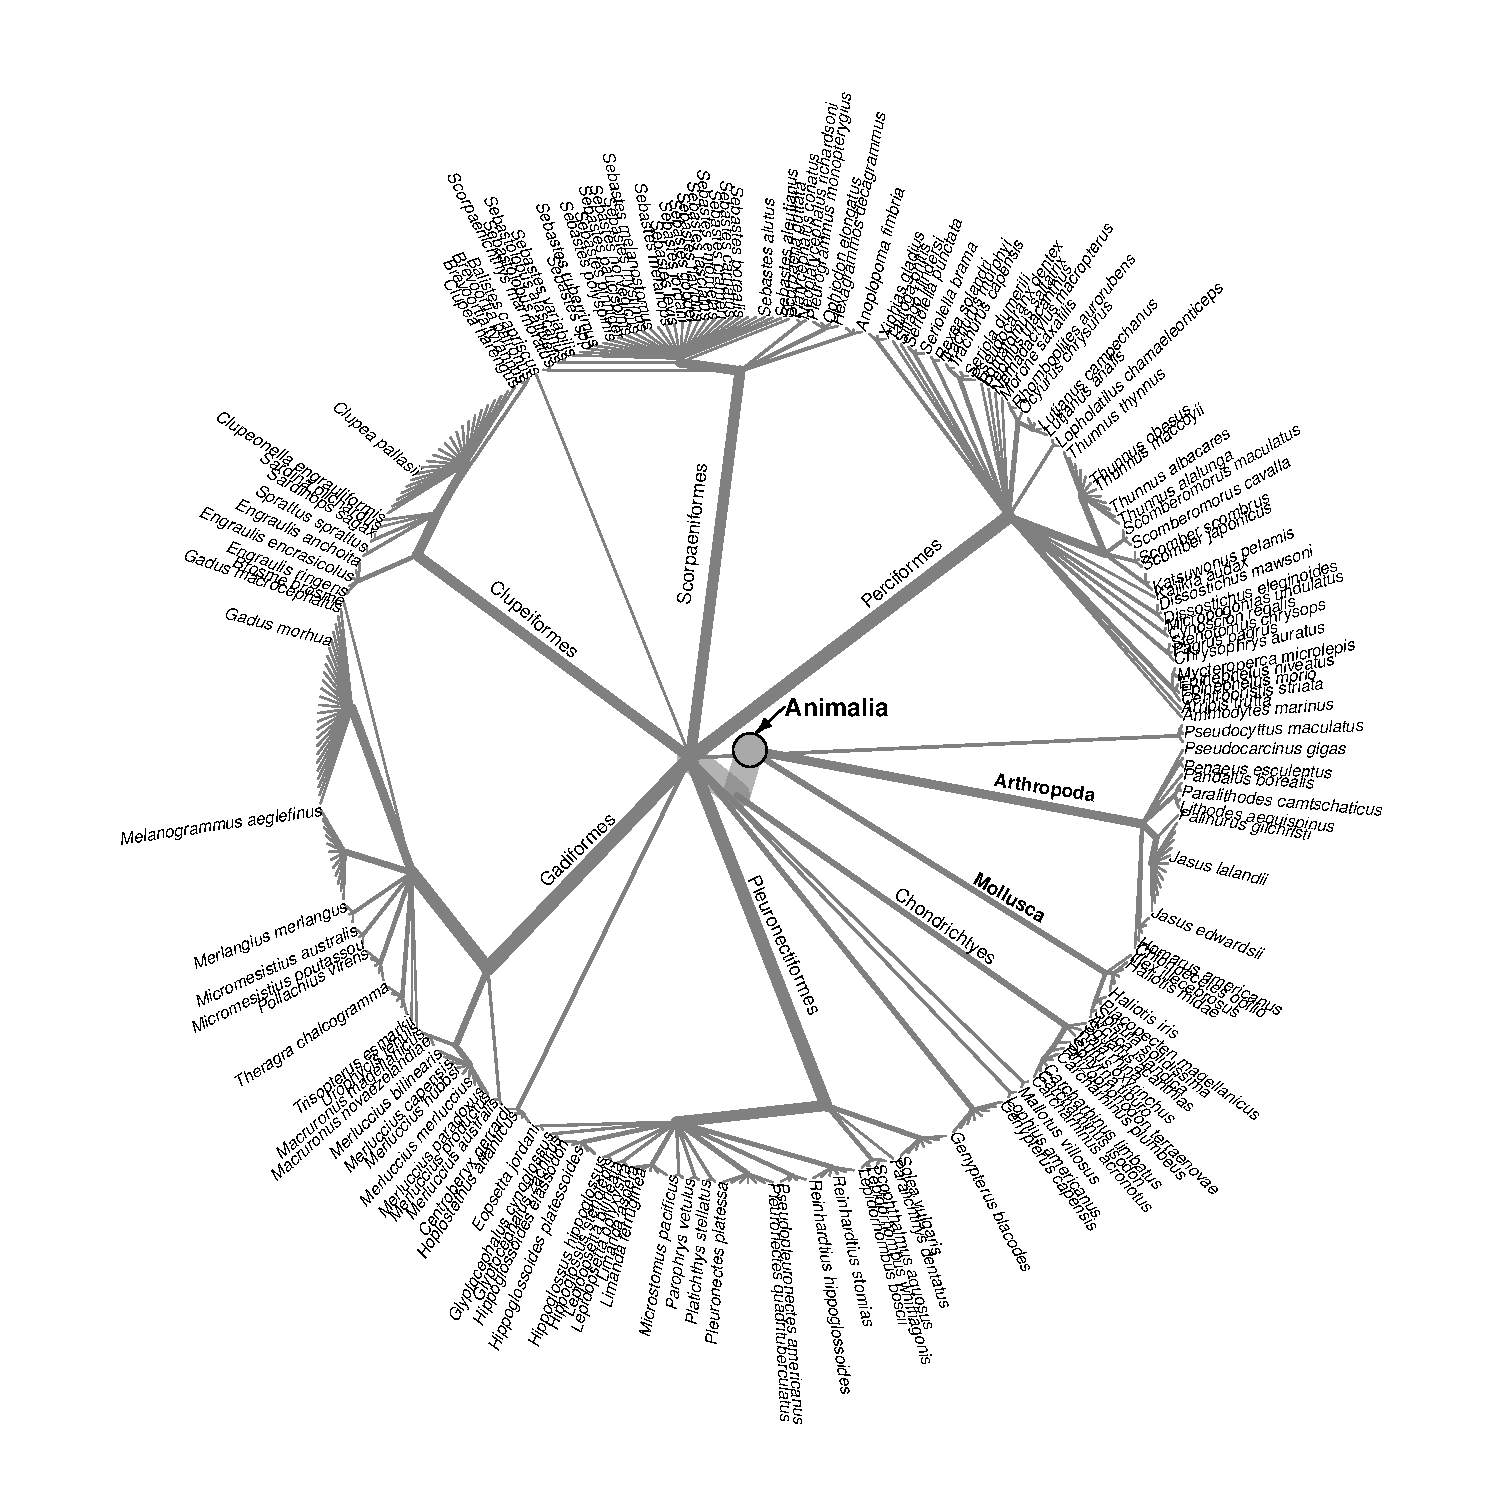
\includegraphics[width=7.5in]{/home/srdbadmin/srdb/projects/fishandfisheries/R/first-review/srdb-by-assessment.pdf} %taxonomic_coverage_byLME.pdf}
\end{center}
\caption{ }\label{fig:taxo:srdb}
\end{figure}


\noindent Figure S3. \\ 

%By taxonomy, inverts and fish, demersal and pelagics  (Figure~\ref{fig:group}).
\begin{figure}
\begin{center}
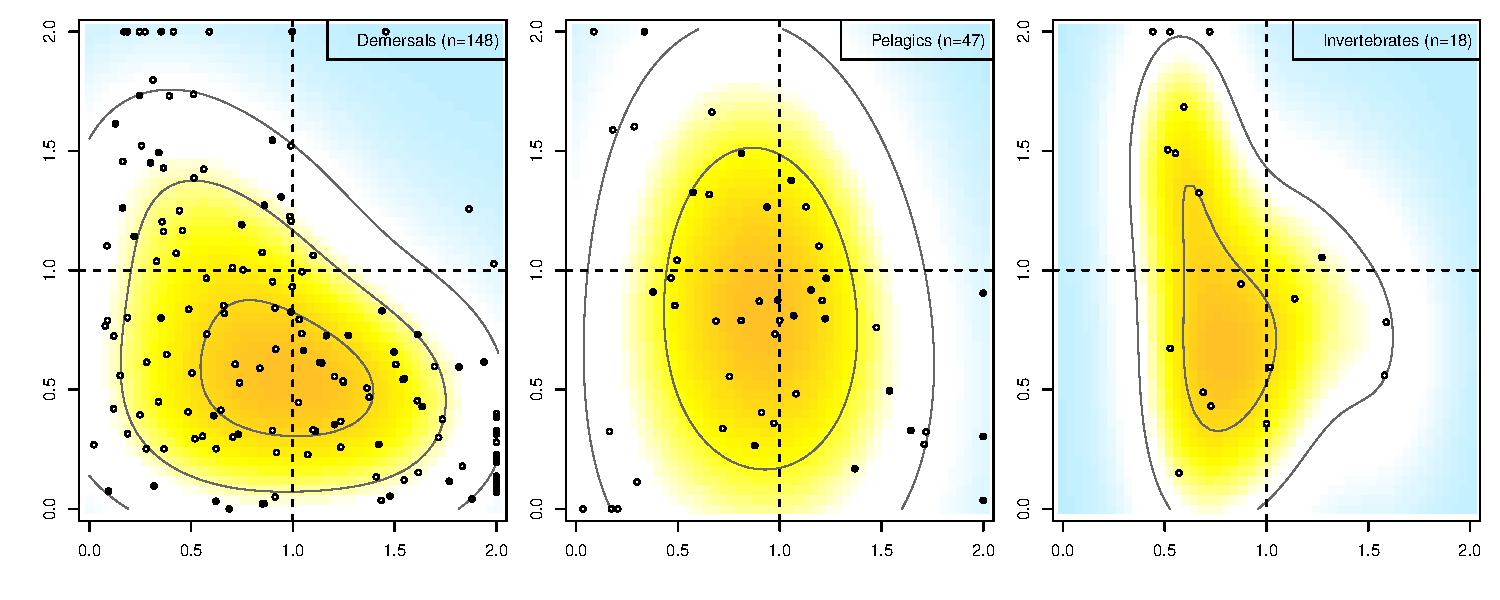
\includegraphics[width=15cm]{/home/srdbadmin/srdb/projects/fishandfisheries/R/first-review/friedegg-bytaxocategory.pdf}
\end{center}
\caption{Invertebrates, demersal fish and pelagic fish.}
\label{fig:group}
\end{figure}


\noindent Figure S4. \\ 

%Fried egg plot for ICES using SSBlim reference points instead of SSBmsy  (Figure~\ref{fig:icesblim}).
\begin{figure}
\begin{center}
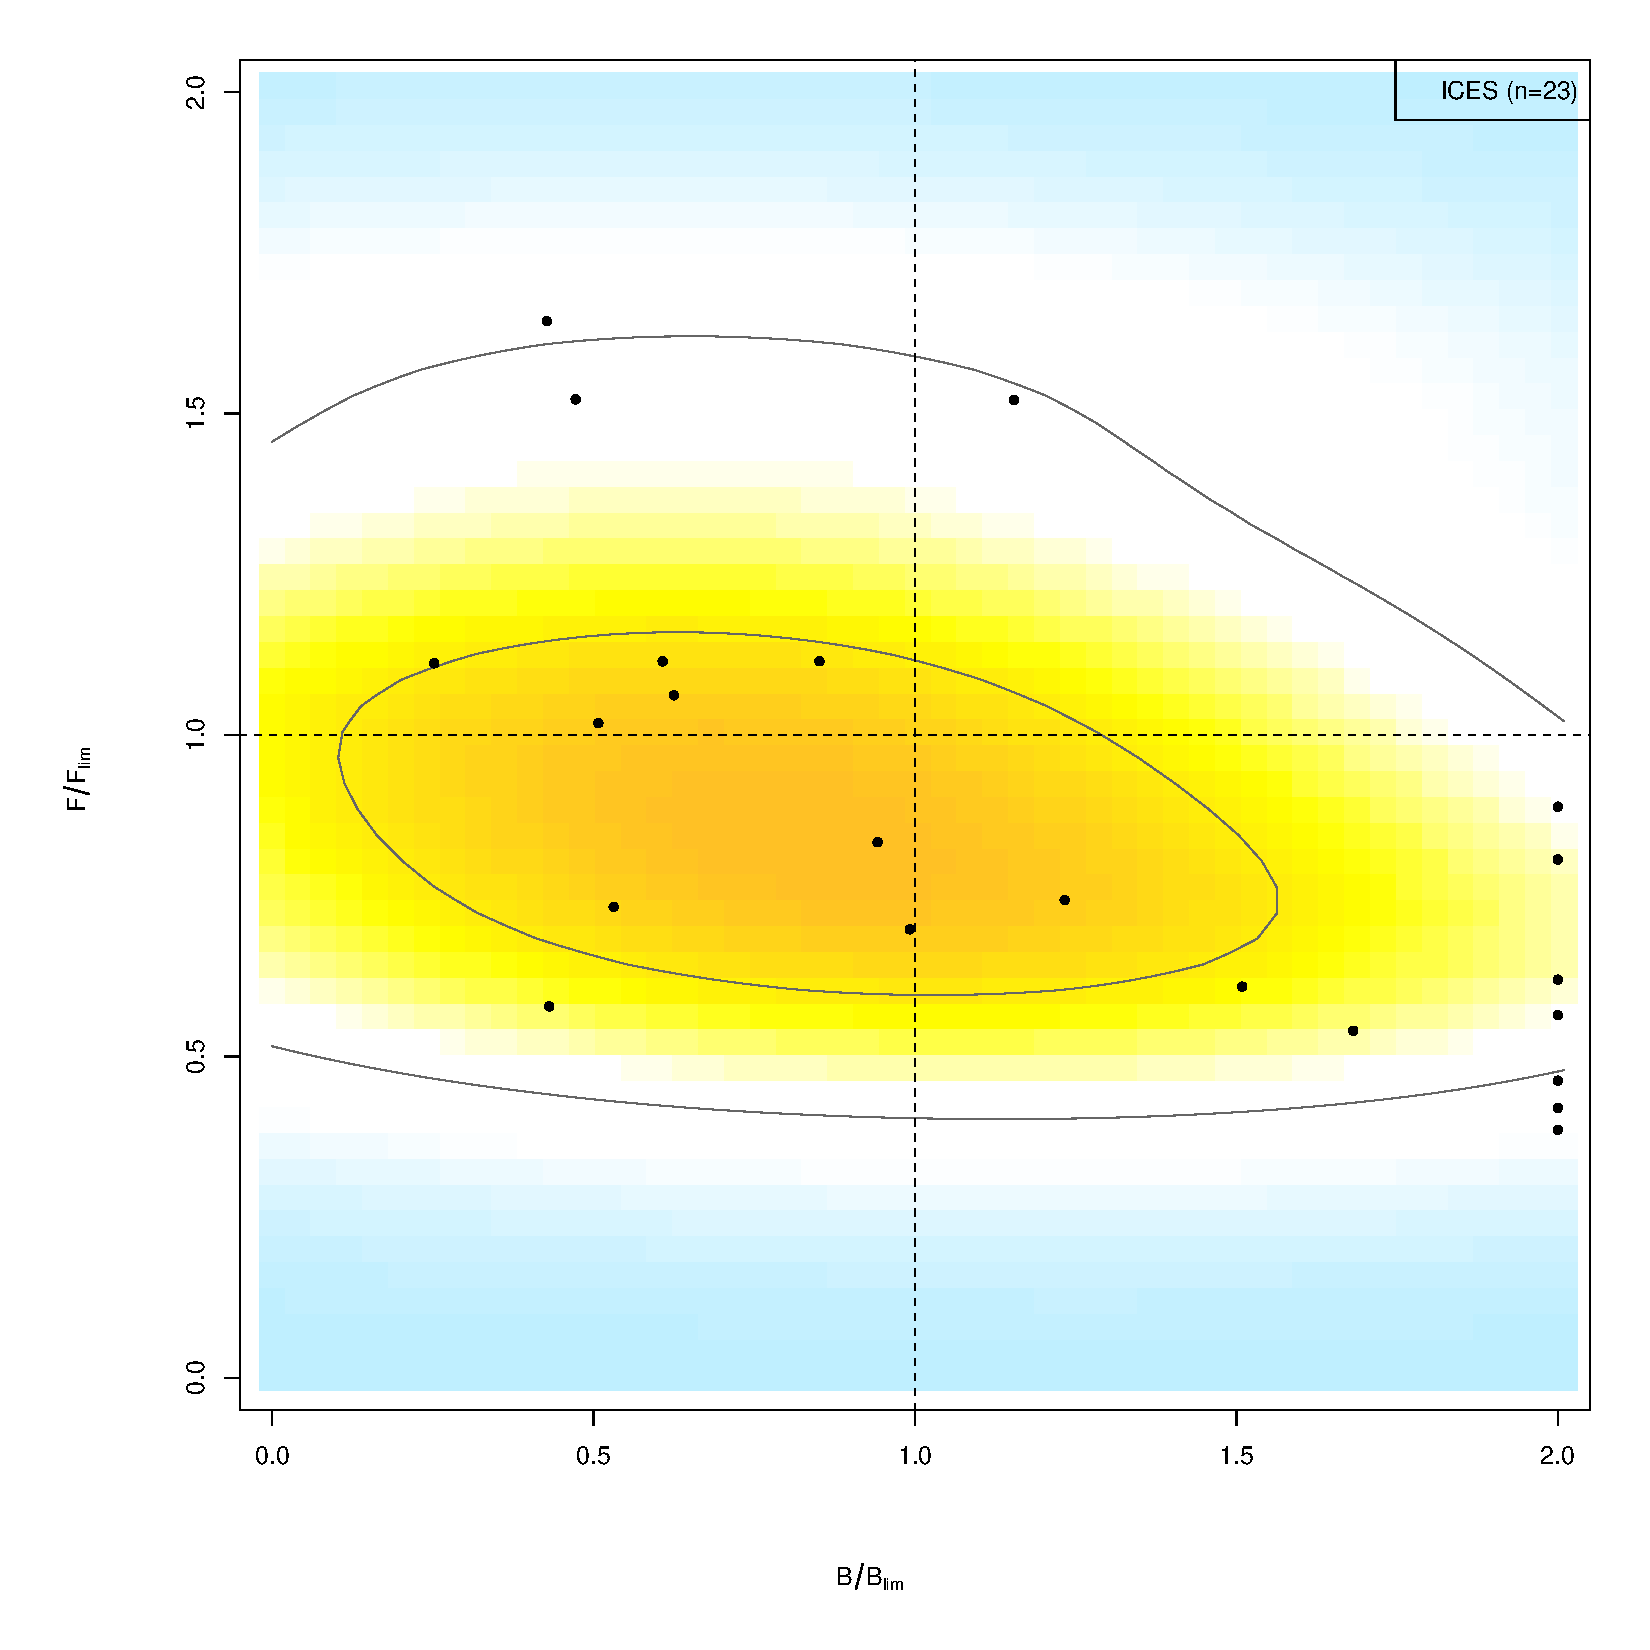
\includegraphics[height=20cm]{/home/srdbadmin/srdb/projects/fishandfisheries/R/first-review/friedegg-ICES-SSBlim.pdf}
\end{center}
\caption{ ICES SSBlim.}
\label{fig:icesblim}
\end{figure}


\noindent Figure S5. \\ 

%Comparison of assessment-derived and Schaefer-derived ratios (Figure~\ref{fig:corr}).
\begin{figure}
\begin{center}
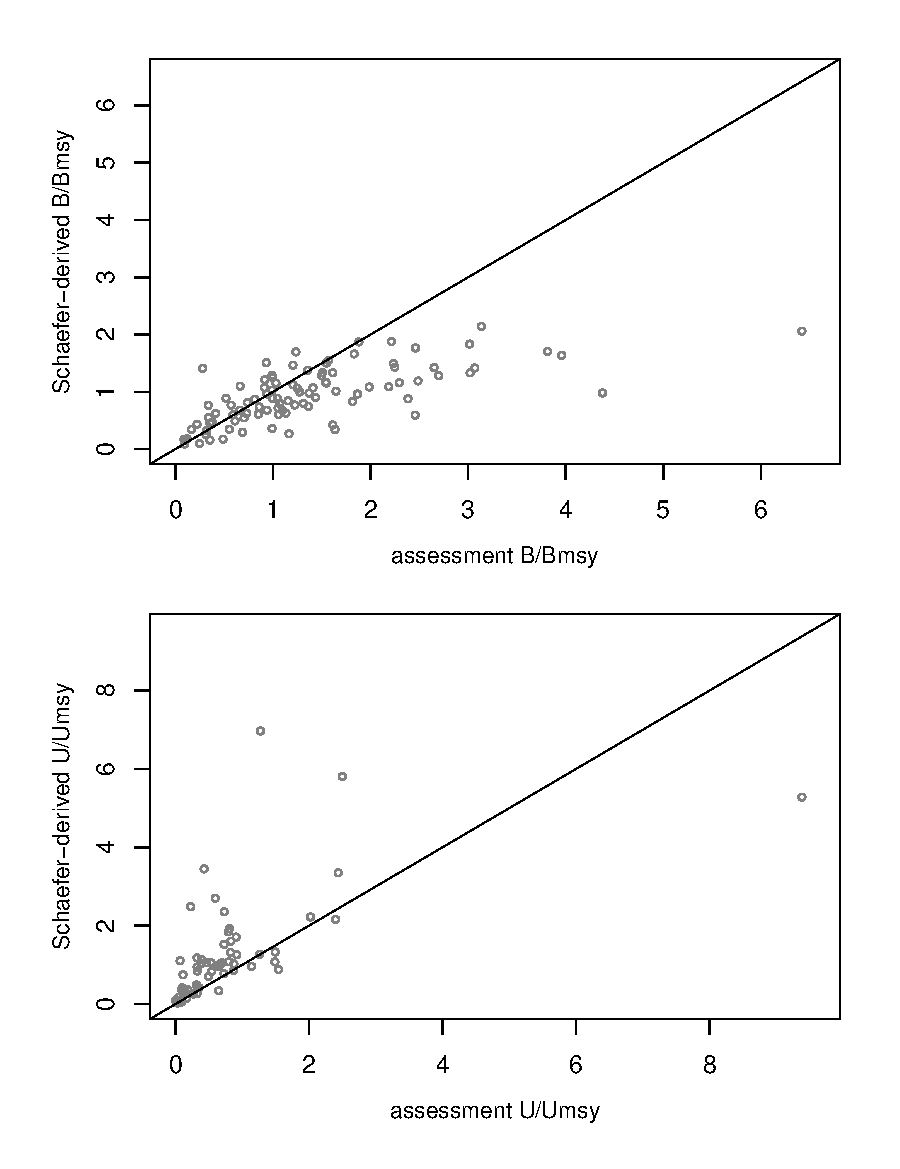
\includegraphics[width=15cm]{/home/srdbadmin/srdb/projects/fishandfisheries/R/first-review/Schaefer-correlations.pdf}
\end{center}
\caption{ }\label{fig:corr}
\end{figure}

% Comparison of ratios for 2 different upper bounds for K

%\noindent Figure S6. \\ 
%\begin{figure}
%\begin{center}
%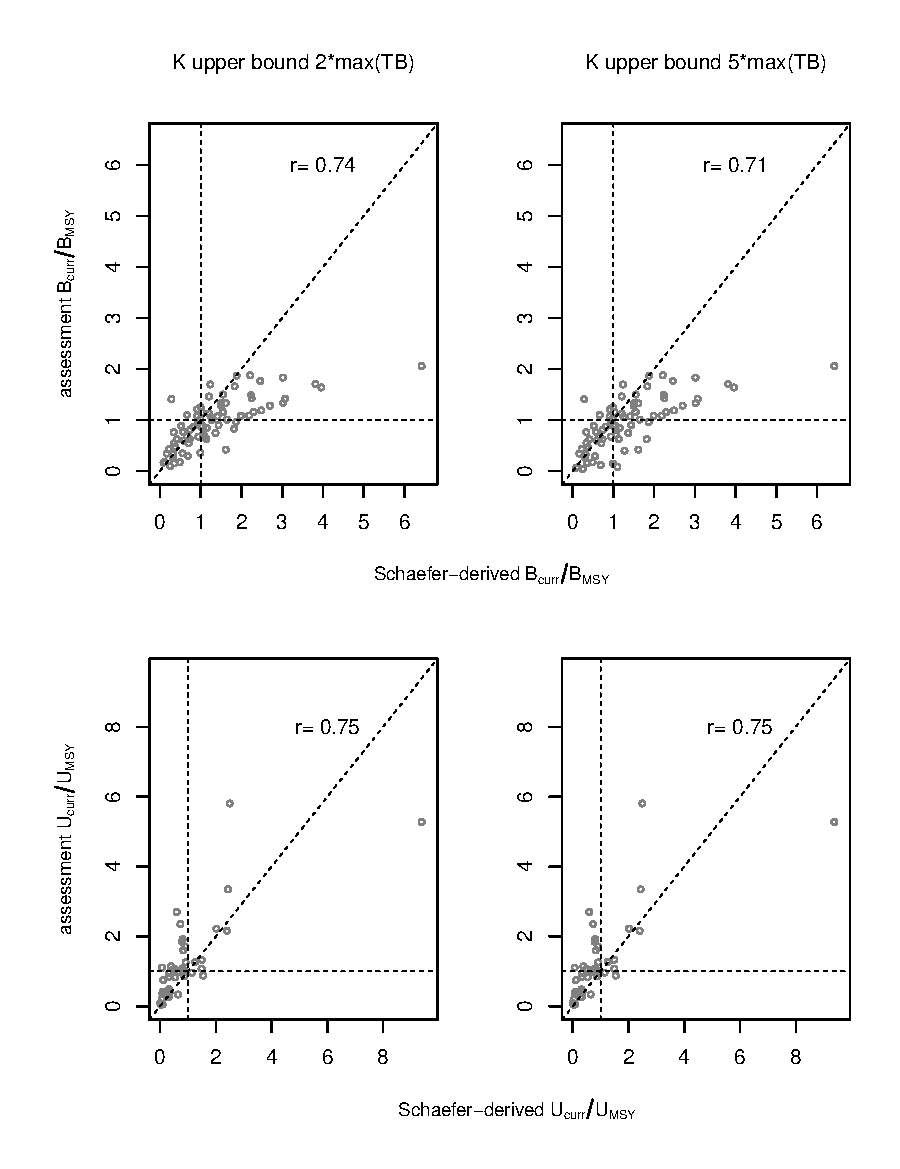
\includegraphics[width=15cm]{/home/srdbadmin/srdb/projects/fishandfisheries/R/first-review/Schaefer-correlations-Kbounds-comparison.pdf}
%\end{center}
%\caption{ }\label{fig:corr:comp}
%\end{figure}


%By LME (Figure~\ref{fig:lme}).
%\begin{figure}
%\begin{center}
%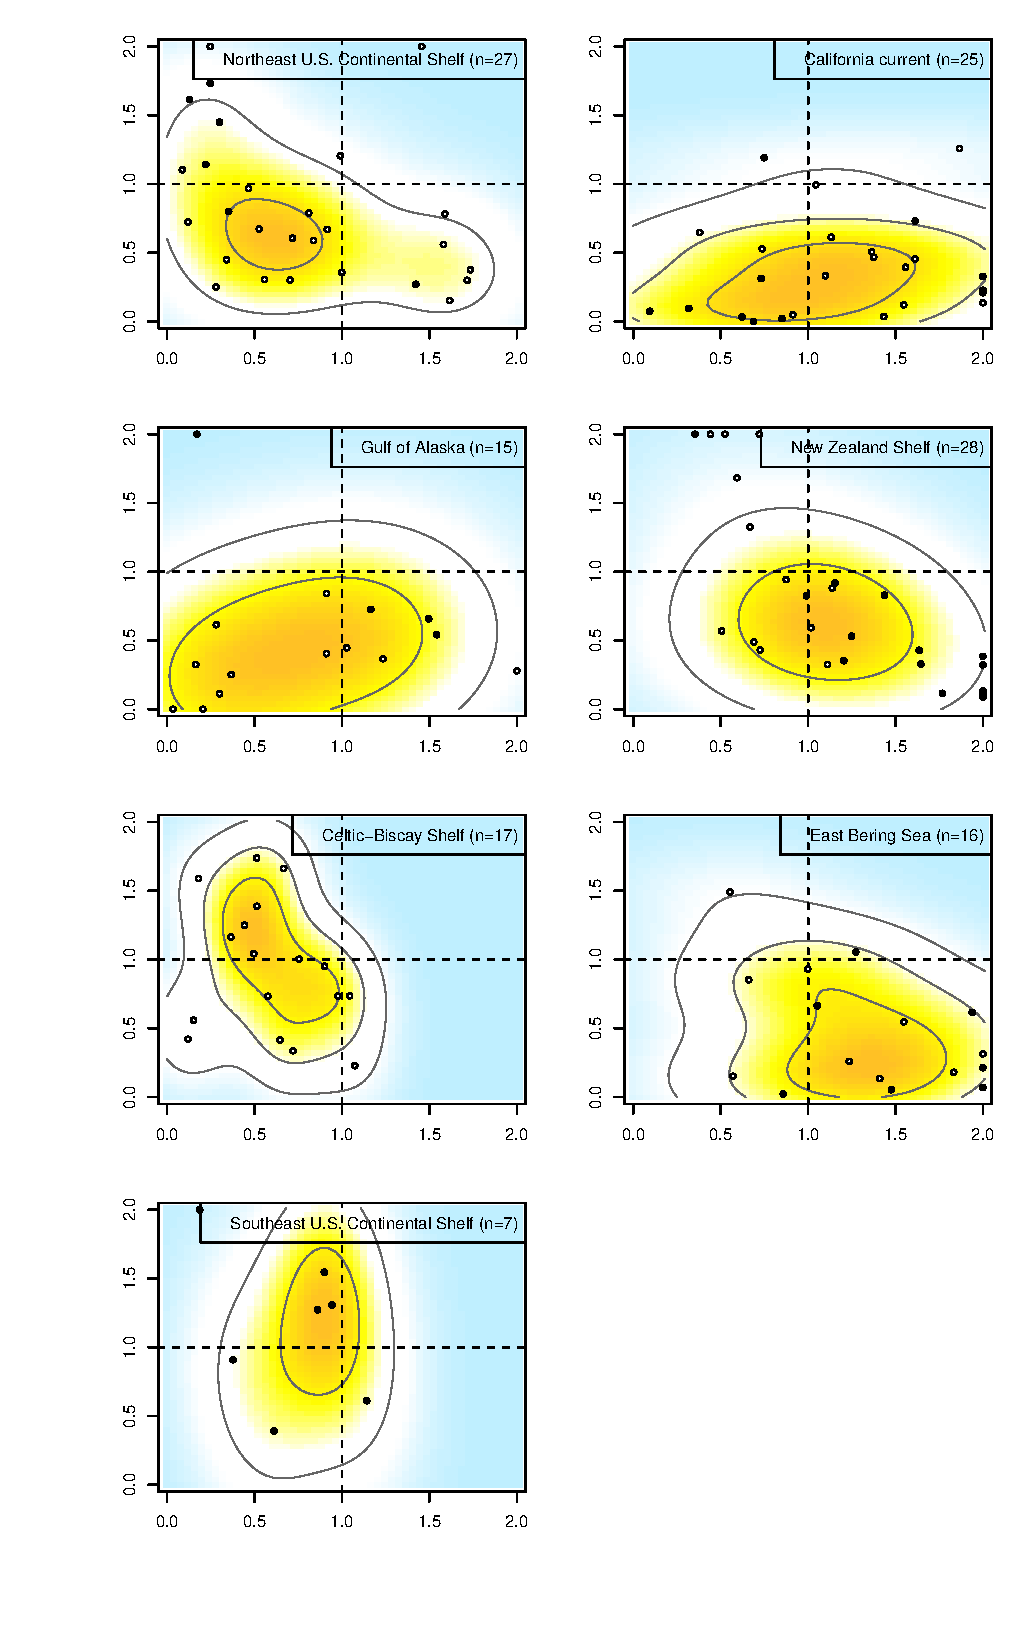
\includegraphics[height=20cm]{/home/srdbadmin/srdb/projects/fishandfisheries/R/first-review/friedegg-LMEs.pdf}
%\end{center}
%\caption{By Large Marine Ecosystem (LME).}
%\label{fig:lme}
%\end{figure}


%By the top 30 fisheries as per Table 2  (Figure~\ref{fig:top30}).
%\begin{figure}
%\begin{center}
%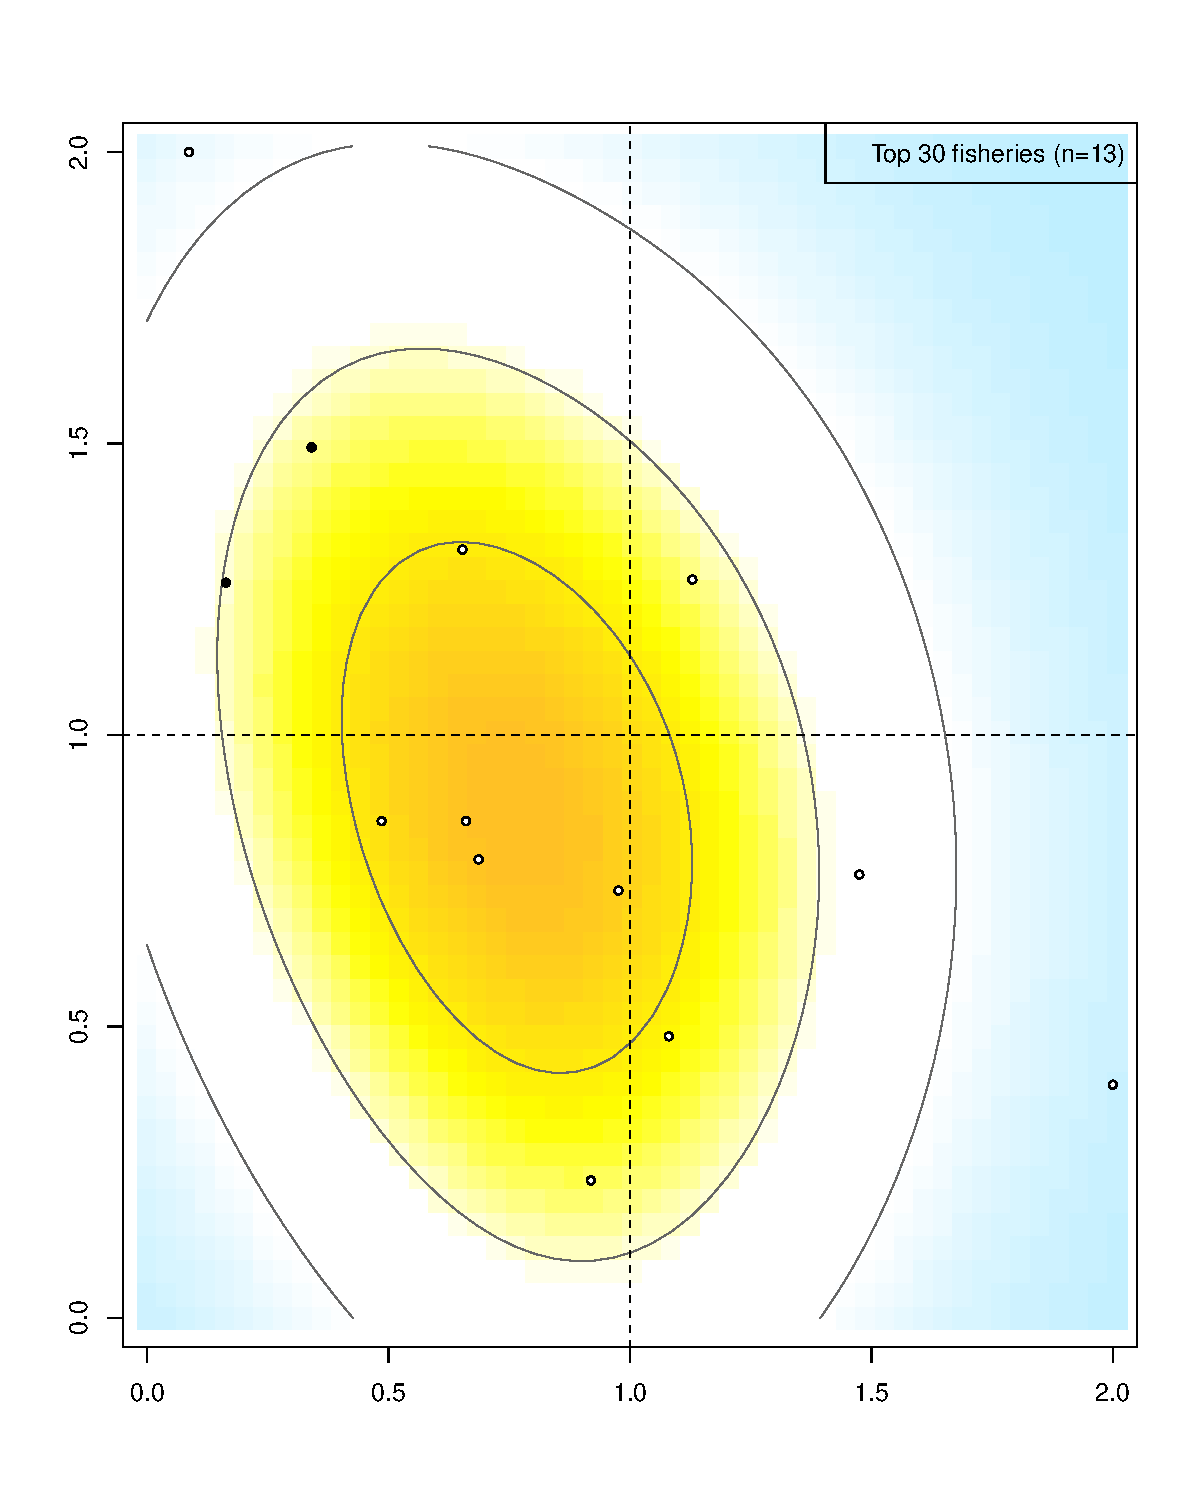
\includegraphics[width=15cm]{/home/srdbadmin/srdb/projects/fishandfisheries/R/first-review/friedegg-top30fisheries.pdf}
%\end{center}
%\caption{ Top 30 fisheries.}
%\label{fig:top30}
%\end{figure}

\end{appendix}
\end{document}

